\documentclass{pracamgr}

\usepackage{polski}   
\usepackage[utf8]{inputenc}
\usepackage[T1]{fontenc}
\usepackage{graphicx} 
\usepackage{amsmath}
%\usepackage{appendix}

\author{Andrzej Żurański}

\nralbumu{WFAIS/Fz/155/03/04}

\title{Algorytm systemu wyzwalania dla radiacyjnych rozpadów mezonów pięknych w eksperymencie LHCb}

\tytulang{\centering High level trigger algorithm for B-meson radiative decays at the LHCb experiment.}

%kierunek: Matematyka, Informatyka, ...
\kierunek{Fizyka Doświadczalna}

% informatyka - nie okreslamy zakresu (opcja zakomentowana)
% matematyka - zakres moze pozostac nieokreslony,
% a jesli ma byc okreslony dla pracy mgr,
% to przyjmuje jedna z wartosci:
% {metod matematycznych w finansach}
% {metod matematycznych w ubezpieczeniach}
% {matematyki stosowanej}
% {nauczania matematyki}
% Dla pracy licencjackiej mamy natomiast
% mozliwosc wpisania takiej wartosci zakresu:
% {Jednoczesnych Studiow Ekonomiczno--Matematycznych}

% \zakres{Tu wpisac, jesli trzeba, jedna z opcji podanych wyzej}

% Praca wykonana pod kierunkiem:
% (podatuopieinazwisko opiekuna
% Instytut
% ew. Wydzia. Uczelnia (je nie MIM UW))
\opiekun{dr hab. Mariusza Witka\\
 z Instytutu Fizyki Jądrowej PAN\\
  }

% miesi~rok:
\date{Czerwiec 2008}

%Podaiedzin klasyfikacji Socrates-Erasmus:
%\dziedzina{ 
%11.0 Matematyka, Informatyka:\\ 
%11.1 Matematyka\\ 
%11.2 Statystyka\\ 
%11.3 Informatyka\\ 
%11.4 Sztuczna inteligencja\\ 
%11.5 Nauki aktuarialne\\
%11.9 Inne nauki matematyczne i informatyczne
%13.2 Fizyka
%}

%Klasyfikacja tematyczna wedlug AMS (matematyka) lub ACM (informatyka)
%\klasyfikacja{D. Software\\
 % D.127. Blabalgorithms\\
  %D.127.6. Numerical blabalysis}

% S kluczowe:
\keywords{system wyzwalania, tryger, separacja $\pi^0/foton$, łamanie CP, eksperyment LHCb, High Level Trigger, Level-0}

\begin{document}
\baselineskip=18pt
\maketitle

%tu idzie streszczenie na strone poczatkowa
\begin{abstract}
Niniejsza praca zawiera opis optymalizacji algorytmów alei fotonowej wysokiego poziomu systemu wyzwalania w eksperymencie LHCb oraz wyniki przeprowadzonej analizy. Pierwotna wersja alei fotonowej działa z 56\% wydajnością dla przypadków sygnałowych (rozpady mezonów \textit{B} z fotonem), jednocześnie całkowita częstotliwość akceptacji wszystkich przypadków wynosi 8 kHz. Wydajność przypadków sygnałowych na poziomie 56\% została zrozumiana i wyjaśniona w pracy. Celem pracy jest poprawienie tych rezultatów tak, aby spełniały wymogi systemu wyzwalania eksperymentu. Konstrukcja systemu wyzwalania eksperymentu LHCb zakłada częstotliwość akceptacji przypadków przez aleję fotonową na poziomie 3 kHz przy możliwie jak najwyższej wydajności dla przypadków sygnałowych. Opracowano algorytm separacji sygnału i tła na podstawie klastrów elektromagnetycznych, który pozwala, stosując separację $\pi^0$/foton z wykorzystaniem metody Fishera, na 3-krotne obniżenie poziomu tła przy 88,7\% wydajności dla fotonowych rozpadów \textit{B}. Zoptymalizowano także sekwencję cięć dla śladów pochodzących od cząstek z rozpadu mezonów \textit{B}. Uzyskano całkowitą efektywność alei na poziomie 64\% dla przypadków sygnału od radiacyjnych rozpadów \textit{B} przy obniżeniu poziomu tła poniżej 3 kHz, zaś dla tła na poziomie 8 kHz uzyskano 75\% wydajności sygnałowej. 
\end{abstract}



\tableofcontents
%\listoffigures
%\listoftables

\chapter*{Wprowadzenie}
\addcontentsline{toc}{chapter}{Wprowadzenie}
\hspace{20pt}Zagadnienie systemu wyzwalania staje się coraz większym wyzwaniem współczesnych wielkich eksperymentów w fizyce cząstek elementarnych. Eksperymenty będące w przygotowaniu dla akceleratora Large Hadron Collider (LHC) znajdującego się w Europejskim Laboratorium Fizyki Cząstek CERN pod Genewą wymagają specjalnego podejścia do systemu wyzwalania. Zderzenia rejestrowane przez detektory w LHC będą dostarczane z częstotliwością 40 MHz (zderzenia następują po sobie co $25\cdot 10^{-9}s$) i nie mogą być zapisane do pełnej analizy z taką częstotliwością. Ograniczony budżet pozwala na zapis rejestrowanych przypadków na nośnikach pamięci jedynie z częstotliwością kilkuset herców. Oznacza to, że częstotliwość przychodzenia przypadków musi zostać obniżona o blisko pięć rzędów wielkości. Z uwagi na fakt, iż celem eksperymentów na LHC jest badanie rzadkich zdarzeń w zderzeniach proton-proton, wyspecjalizowany system wyzwalania i zapisu przypadków jest wymagany w celu selekcji najciekawszych z fizycznego punktu widzenia przypadków. Systemy wyzwalania, obecnie konstruowane wielostopniowo, wymagają szybkiej analizy przypadków w czasie rzeczywistym. Dlatego też ich konstrukcja i efektywność działania są kluczowym elementem tych eksperymentów.
\\
\indent
Jednym z eksperymentów przeprowadzanych na LHC będzie LHCb (\textit{Large Hadron Collider Beauty Experiment}), który jest dedykowanym eksperymentem do badania fizyki cząstek zawierających kwark piękny \textit{b}. Fizyka kwarków \textit{b} jest szczególnie interesująca pod kątem badania łamania parzystości kombinowanej CP oraz rzadkich rozpadów mezonów pięknych. Badania w tym kierunku mogą znacząco przyczynić się do wyjaśnienia obecnie obserwowanej asymetrii pomiędzy materią a antymaterią we wszechświecie. Jednym z zadań eksperymentu LHCb jest badanie rzadkich rozpadów mezonów pięknych z fotonem w stanie końcowym, tzw. rozpadów radiacyjnych. W tym celu w konstrukcji systemu wyzwalania znajduje się specjalna część dedykowana selekcji tych właśnie rozpadów. Ponieważ ogromną większość zdarzeń w eksperymencie LHCb stanowią przypadki nieinteresujące, poniższa praca jest poświęcona opracowaniu algorytmów selekcji rozpadów radiacyjnych mezonów \textit{B} dających wymaganą redukcję częstotliwości przychodzenia przypadków nieinteresujących.
\\
\indent
Praca została wykonana w Instytucie Fizyki Jądrowej PAN w Krakowie pod kierunkiem doktora habilitowanego Mariusza Witka, któremu pragnę serdecznie podziękować za okazaną pomoc i opiekę dydaktyczną podczas powstawania pracy. Opracowane algorytmy alei fotonowej wysokiego stopnia systemu wyzwalania zostaną w niedalekiej przyszłości wykorzystane na potrzeby eksperymentu LHCb.




\chapter{Wstęp}
\addcontentsline{toc}{chapter}{Wstęp}

\section{Eksperyment LHCb w CERN-ie}

Eksperyment LHCb będzie przeprowadzony w Europejskim Laboratorium Fizyki Cząstek (CERN) w Genewie na budowanym obecnie dużym akceleratorze protonowym wiązek przeciwbieżnych - Large Hadron Collider (LHC). 
Bierze w nim udział ok. 50 laboratoriów z całego świata. Ze strony polskiej oprócz Instytutu Fizyki Jądrowej PAN uczestniczą w nim jeszcze Instytut Problemów Jądrowych (IPJ) oraz Akademia Górniczo-Hutnicza (AGH). Program fizyczny eksperymentu obejmuje badanie łamania tzw. parzystości kombinowanej (CP) w procesach rozpadu cząstek zawierających kwark piękny \textit{b}, głównie mezonów $B$ i $B_s$ oraz poszukiwania ich rzadkich rozpadów. Rozpoczęcie zbierania danych przewiduje się w momencie uruchomienia akceleratora LHC tzn. na jesieni 2008 r.
\\
%\subsection{Detektor eksperymentu}

\noindent
Akcelerator LHC będzie zderzał ze sobą przeciwbieżne wiązki protonów o energii 7 TeV w postaci pęczków (ok. $10^{11}$ protonów w pęczku). Dla celów eksperymentu LHCb świetlność w punkcie zderzenia jest obniżona do wartości $2\cdot 10^{32} cm^{-2}s^{-1}$ w stosunku do maksymalnej świetlności akceleratora LHC równej $10^{34} cm^{-2}s^{-1}$.  Przy takiej energii i świetlności w eksperymencie LHCb w przecięciach pęczków dominować będą pojedyncze zderzenia proton-proton. Ma to kluczowe znaczenie w rekonstrukcji pierwotnych i wtórnych wierzchołków oddziaływania, ważnych z punktu widzenia analizy przypadków zawierających mezony \textit{B}.
\\\\
\noindent
Zderzenia w akceleratorze LHC będą zachodziły z częstotliwościa 40 MHz (zderzenia co 25 ns), jednakże dla LHCb częstotliwość przychodzenia przypadków widocznych dla detektora to około 10 MHz (pozostałe zdarzenia są niewidoczne ponieważ ich produkty lecąc pod małymi kątami wpadają w rurę akceleratora). Spośród wszystkich zdarzeń widocznych w detektorze LHCb spodziewanych jest ok. 100 kHz przypadków gdzie w zderzeniu wyprodukowana zostanie para $b\bar{b}$. Jednakże tylko ok. 15\% spośród tych przypadków będzie zawierało wszystkie produkty rozpadu przynajmniej jednego mezonu \textit{B} w obrębie akceptancji detektora (stożek o kącie rozwarcia ok. 400 mrad). Ponieważ stosunki rozpadów mezonów \textit{B} służące do analizy łamania symetrii CP występują zazwyczaj na poziomie $10^{-4}$, koniecznym jest zastosowanie wyspecjalizowanego systemu wyzwalania do selekcji przypadków w trakcie zbierania danych, tzw. trygera [3], który będzie szerzej omówiony w rozdziale 2.
\\\\
\noindent
Detektor eksperymentu LHCb jest jednoramiennych spektrometrem obejmującym zakres pseudorapidity\footnote{pseudorapidity $\eta=-log(tg(\frac{\theta}{2}))$ jest zmienną geometryczną w układzie laboratoryjnym. $\theta$ jest kątem nachylenia do osi akceleratora, a początek układu laboratoryjnego znajduje się w punkcie zderzenia pęczków protonowych.} $1.9 < \eta < 4.9$. Spektrometr pokazany na rysunku 1.1 składa się z następujących części [4]:
\begin{itemize}
 \item[-] Vertex Locator (VELO) - krzemowy detektor wierzchołka służący do rekonstrukcji wierzchołka pierwotnego i wierzchołków wtórnych
 \item[-] Trigger Tracker (TT) - detektor śladowy umieszczony za detektorem VELO
 \item[-] detektory Ring Imaging Cherenkov (RICH 1 i 2) - detektory Czerenkowa służące do identyfikacji cząstek (protonów, kaonów, pionów)
 \item[-] T1-T3 - stacje detektorów śladowych służące do rekonstrukcji trajektorii cząstek po przejściu przez pole magnetyczne 
 \item[-] kalorymetr elektromagnetyczny (ECAL) - służy do pomiaru energii cząstek oddziaływujących elektromagnetycznie: fotonu, elektronu, mezonu $\pi^0$ etc.
 \item[-] kalorymetr hadronowy (HCAL) - służący do pomiaru energii hadronów
 \item[-] stacje mionowe - służące do identyfikacji i pomiaru pędu mionów
\end{itemize}

\begin{figure}[h!]
 \centering
 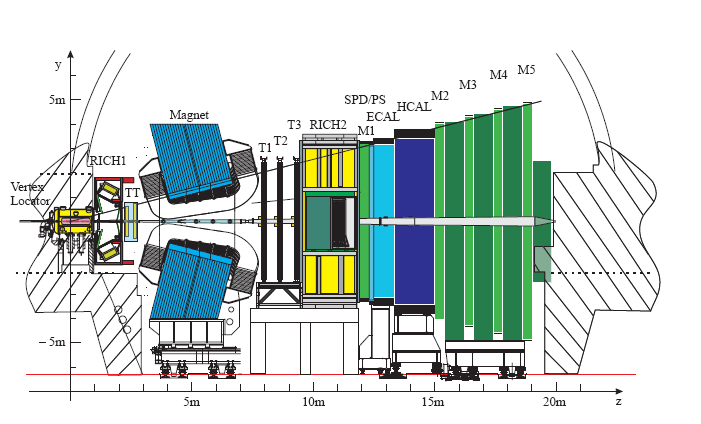
\includegraphics[width=1.0\textwidth]{rysunki/introduction/det1.png}
 \caption{Detektor LHCb w rzucie y-z.}
\end{figure}

\section{Główne cele eksperymentu}

Głównym celem eksperymentu jest badanie naruszania symetrii CP tzw. parzystości kombinowanej\footnote{Transformacja CP polega na kolejnym wykonaniu operacji sprzężenia ładunkowego C i inwersji przestrzennej $r \rightarrow -r$. Sens fizyczny tej transformacji jest taki, że przeprowadza ona stan spolaryzowanej lewo- lub prawoskrętnie cząstki w stan spolaryzowanej prawo- lub lewoskrętnie antycząstki.} (efektu odkrytego w latach 60-tych w rozpadach długożyciowych mezonów $K^{0}$)[1]. W Modelu Standardowym można uwzględnić to zjawisko przez odpowiednią parametryzację macierzy CKM (nazwa pochodzi od nazwisk autorów Cabbibo, Kobayashi, Maskawa) (rys. 1.2), opisującą przejścia pomiędzy trzema rodzinami kwarków jako skutek ich oddziaływania z nośnikami słabych oddziaływań, bozonami $W^{\pm}$. Macierz ta posiada jedną zespoloną fazę, która jest miarą łamania parzystości CP dla mieszania kwarków. Wszystkie elementy macierzy CKM trzeba wyznaczyć z doświadczenia. Teoria przewiduje tylko pewne związki pomiędzy tymi elementami w postaci trójkątów unitarności (rys 1.3).
\\

\begin{figure}[h!]
 \hspace{20pt}a) \hspace{160pt} b)
\begin{center}
 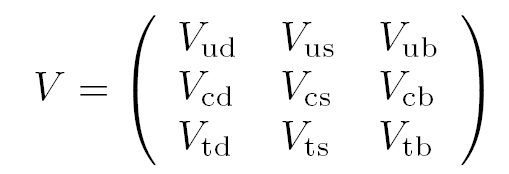
\includegraphics[width=0.35\textwidth]{rysunki/introduction/ckm1.png}
 \hspace{5pt}
 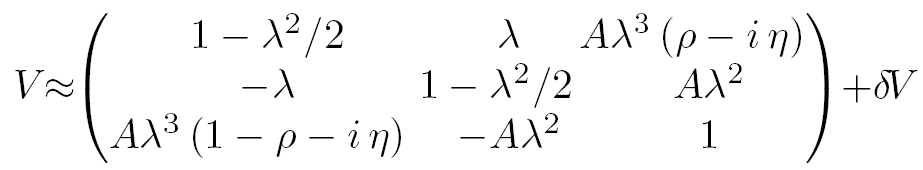
\includegraphics[width=0.55\textwidth]{rysunki/introduction/ckm2.png}
 \caption{Macierz CKM mieszania kwarków przez prądy naładowane (a), macierz CKM po zastosowaniu parametryzacji Wolfensteina (b).}
\end{center}
\end{figure}

\begin{figure}[h!]
 \centering
 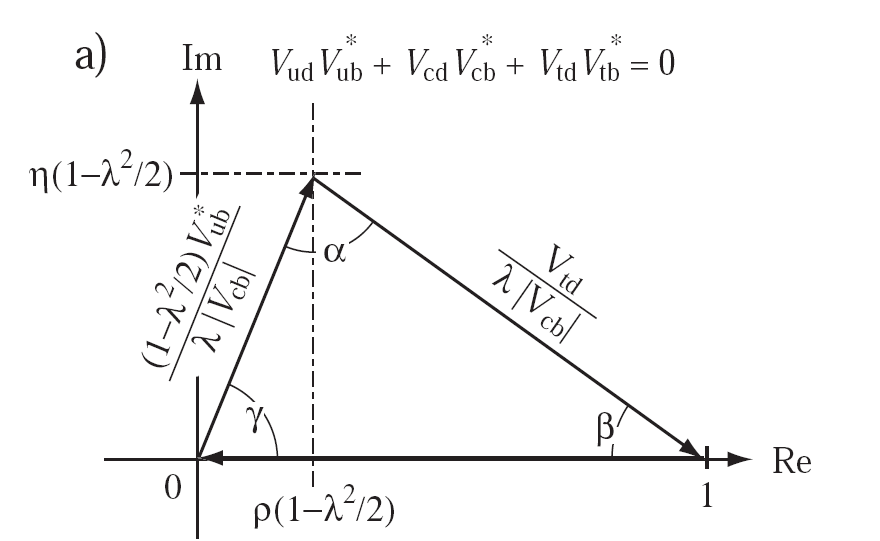
\includegraphics[width=0.45\textwidth]{rysunki/introduction/trojkat1.png}
 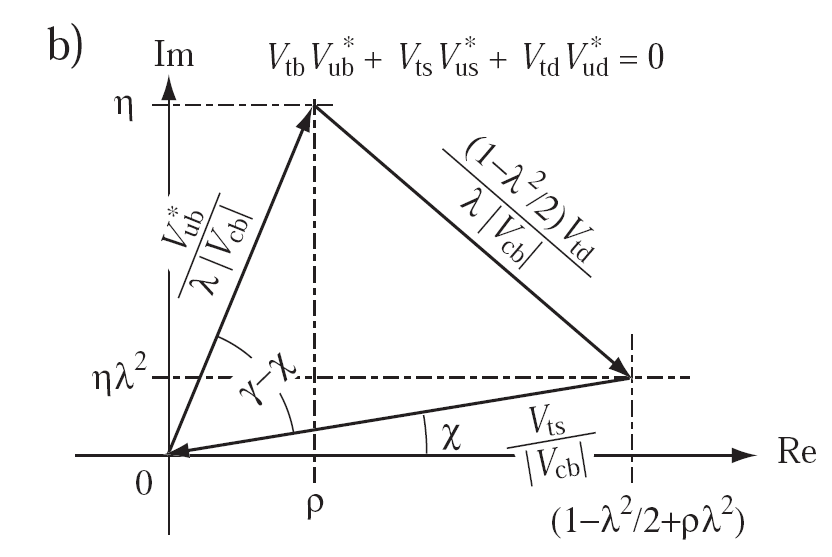
\includegraphics[width=0.45\textwidth]{rysunki/introduction/trojkat2.png}
 \caption{Trójkąty unitarności macierzy CKM.}
\end{figure}

\noindent Poznanie źródeł łamania parzystości CP jest także ważne dla zrozumienia istniejącej we wszechświecie przewagi ilości materii nad ilością antymaterii. Proponowany mechanizm prowadzący od wszechświata z taką samą liczbą cząstek i antycząstek do obserwowanej obecnie asymetrii wymaga jednak znacznie większego niż w Modelu Standardowym stopnia łamania symetrii CP. Stąd bierze się przypuszczenie, że mechanizm Modelu Standardowego nie jest jedynym źródłem łamania CP i badania tego zjawiska doprowadzą do odkrycia procesów wykraczajacych poza ten model - do tzw. nowej fizyki. Program testowania mechanizmu łamania parzystości CP w Modelu Standardowym i poszukiwania ewentualnych odstępstw od przewidywań tej teorii wymaga bardzo dokładnych pomiarów dla możliwie dużej liczby różnych rozpadów cząstek pięknych, dlatego też im więcej zbadanych rozpadów tym więcej ograniczeń nakładanych na wyznaczane parametry modelu. Tabela 1.1 pokazuje spodziewaną liczbę zebranych przypadków w poszczególnych kanałach rozpadów mezonów pięknych dla eksperymentu LHCb.

\begin{table}[h!]
\centering
 \caption{Przykłady kanałów rozpadu mezonów $B^{0}$ i ich względne częstości rozpadu. Mezony $B^{0}_{d}$ składają się z kwarka $d$ i antykwarka $\bar{b}$, a mezony $B^{0}_{s}$ z kwarka $s$ i antykwarka $\bar{b}$. Podano przewidywane liczby zrekonstruowanych rozpadów mezonów \textit{B} zebranych w ciągu jednego roku ($10^7$ s) pracy detektora LHCb przy założeniu średniej świetlności $2\cdot 10^{32} cm^{-2}s^{-1}$.}
 \vspace{5pt}
 \begin{tabular}{lcr}
  \hline\hline
   & & \\
  Kanał rozpadu & \hspace{5pt} Względna częstość rozpadu & Liczba zrekonstruowanych przypadków \\
   & & w eksperymencie LHCb (1 rok = $10^{7}$ s)\\
   & & \\
  \hline
   & & \\ 
  $B^{0}_{d}\rightarrow J/\psi K^{0}_{s}$ & $4,4\cdot 10^{-4}$ & 56 000\hspace{80pt} \\
  $B^{0}_{d}\rightarrow \pi^{+}\pi^{-}$ & $0,7\cdot 10^{-5}$ & 5000\hspace{80pt} \\
  $B^{0}_{d}\rightarrow \rho^{+}\pi^{-}$ & $1,8\cdot 10^{-5}$ & 1000\hspace{80pt} \\
  $B^{0}_{d}\rightarrow D^{*-}\pi^{+}$ & $2,6\cdot 10^{-3}$ & 340 000\hspace{80pt} \\
%  $B^{0}_{d}\rightarrow \bar{D}^{0}K^{*}$ & $1,3\cdot 10^{-5}$ & 500\hspace{80pt} \\
   & & \\
  \hline
   & & \\
  $B^{0}_{s}\rightarrow J/\psi \phi$ & $9,3\cdot 10^{-4}$ & 44 000\hspace{80pt} \\
  $B^{0}_{s}\rightarrow K^{+}K^{-}$ & $1,5\cdot 10^{-5}$ & 6500\hspace{80pt} \\
  $B^{0}_{s}\rightarrow D^{-}_{s}K^{+}$ & $2,0\cdot 10^{-4}$ & 2400\hspace{80pt} \\
   & & \\
  \hline\hline
 \end{tabular}
\end{table}

%\newpage
\section{Cechy fizyczne radiacyjnych rozpadów mezonów B}

Badanie radiacyjnych rozpadów mezonów pięknych będąc precyzyjnym testem Modelu Standardowego może jednocześnie dostarczyć wielu informacji o interesujących nas odstępstwach od obecnej teorii. Ponieważ rozpady te wymagają zmiany zapachu kwarku poprzez prądy neutralne ich amplitudy są czułe na nowe efekty (stałe sprzężenia) spoza Modelu Standardowego.
\\\\
\noindent
Jedną z metod poszukiwania nowych zjawisk jest systematyczne badanie łamania parzystości kombinowanej CP w rozpadach radiacyjnych mezonów \textit{B} (termin mezony \textit{B} odnosi się tutaj do $B_d$ i $B_s$). W tym wypadku symetria CP może zostać złamana na dwa różne sposoby [2]:
\begin{itemize}
 \item bezpośrednie łamanie CP - polega na istnieniu różnicy w amplitudach rozpadów $B\rightarrow X \gamma$ i $\bar{B}\rightarrow \bar{X}\gamma$ (kreska nad stanem cząstkowym oznacza jego sprzężenie CP); w Modelu Standardowym (MS) bezpośrednie łamanie CP w procesie $b\rightarrow s\gamma$ jest mniejsze niż 1\%, w procesie $b\rightarrow d\gamma$ mniejsze niż 16\%, jednakże w niektórych rozszerzeniach MS wpływ istnienia nowych cząstek może wzmocnić ten efekt do poziomu 10-40\%,
 \item łamanie w wyniku oscylacji $B^{0}_{(s)}-\bar{B^{0}_{(s)}}$ - pojawia się gdy oba stany mogą się rozpaść na taki sam stan końcowy $X^{0}\gamma$ ($X^{0}$ jest nieodróżnialne od $\bar{X^{0}}$), w takich przypadkach ma miejsce interferencja pomiędzy dwoma amplitudami dla rozpadów ze zmianą zapachu w efekcie oscylacji i bez zmiany zapachu. W dotychczasowych badaniach oscylacji mezonów \textit{B} (poszukiwania przeprowadzono w kanale $B^{0}_{d}\rightarrow K^{*}\gamma$) nie zaobserwowano łamania CP, co jest zgodne z przewidywaniami Modelu Standardowego, jednakże w eksperymencie LHCb poszukiwanie łamania CP będzie możliwe w oparciu także o inne kanały rozpadu takie jak $B^{0}\rightarrow \rho^{0}\gamma$ czy $B^{0}_{s}\rightarrow \phi\gamma$.
\end{itemize}
\noindent
Radiacyjne rozpady mezonów pięknych pozwalają także na wyznaczenie stosunku elementów macierzy CKM $|V_{td}/V_{ts}|$. Stosunek ten może być otrzymany za pomocą pomiaru względnej częstości rozpadów 
 $B^{0}\rightarrow \rho^{0}\gamma$ i $B^{0}\rightarrow K^{*}\gamma$.
\\\\
\noindent
Eksperyment LHCb ma na celu uzupełnienie istniejących obserwacji poprzez analizę radiacyjnych rozpadów mezonów $B^{0}_{s}$, a także znaczne poprawienie precyzji obecnych wyników przez pomiar łamania CP w rozpadach zawierających przejścia $b\rightarrow d\gamma$.

\chapter{System wyzwalania}
\addcontentsline{toc}{chapter}{System wyzwalania}

\section{System wyzwalania eksperymentu LHCb}
System wyzwalania (dalej zwany także trygerem) jest kluczowym elementem eksperymentu LHCb. Ma on na celu wybranie do dalszej analizy ciekawych z punktu widzenia analizy fizycznej przypadków, a jednocześnie efektywne odrzucanie przypadków nieinteresujących. Przypadki widziane przez detektor LHCb pojawiają się z częstotliwością 10 MHz co jest związane z parametrami akceleratora (jego świetlnością w punkcie zderzenia oraz całkowitym nieelastycznym przekrojem czynnym na zderzenia pp), jednakże projekt eksperymentu pozwala na zapisanie przypadków na nośnikach pamięci z maksymalną częstotliwością ok. 2 kHz, gdzie wśród przypadków zapisanych powinno się znajdować jak najwięcej interesujących nas rozpadów mezonów \textit{B}. Ograniczenie na częstotliwość zapisywanych do pełnej rekonstrukcji i analizy przypadków spowodowane jest ograniczeniem przepustowości systemu zapisu oraz dostępną do zapisania pamięcią, która przekłada się na koszty całego przedsięwzięcia. W praktyce dla LHCb działanie trygera ma na celu obniżenie częstotliwości przypadków o czynnik 5000, dbając jednocześnie o wysoką efektywność selekcji dla rzadkich rozpadów mezonów \textit{B}.
\\\\
\noindent
Tryger eksperymentu LHCb został zaprojektowany dwustopniowo, co oznacza że selekcja odbywa się na dwóch poziomach niskim i wysokim. Takie rozwiązanie jest podyktowane ograniczeniami czasowymi. Pierwszy stopień tryger (Level-0 dalej zwany L0) analizuje wszystkie przypadki korzystając tylko z bardzo ograniczonej informacji o przypadku (wykorzystywane są detektory, które działają najszybciej) i ma za zadanie odrzucenie części przypadków, tak aby następny wysoki stopień trygera (High Level Trigger dalej zwany HLT) miał więcej czasu na częściową rekonstrukcję przypadku w oparciu o pełną informację z całego detektora, jego analizę i podjęcie decyzji o zapisaniu. Wysoki poziom trygera jest podzielony na dwie główne części. HLT1 obejmuje inkluzywną selekcję przypadków poprzez potwierdzenie słuszności decyzji L0, natomiast drugi etap HLT2 przeprowadza ekskluzywną selekcję poszczególnych kanałów rozpadu. Wielostopniowa konstrukcja ma na celu odrzucanie pewnej części przypadków pozostawiając więcej czasu na coraz dogłębniejszą analizę przypadków akceptowanych. Szczegółowe zasady działania poszczególnych elementrów trygera zostaną opisane w paragrafach 2.1.1 (L0) i 2.1.2 (HLT).

\subsection{Niski poziom trygera - L0}
L0 jest pierwszym stopniem systemu wyzwalania wykonywanym na każdym przychodzącym do detektora przypadku. Jest to tryger sprzętowy całkowicie zsynchronizowany z akceleratorem LHC. Jego działanie ma na celu obniżenie częstotliwości przypadków z początkowej wartości 10 MHz do 1 MHz. Jeśli przypadek otrzyma pozytywną decyzję L0, to będzie dalej analizowany przez wysoki poziom trygera HLT. Ze względu na ograniczony czas dostępny od momentu zajścia zderzenia do podjęcia decyzji algorytm L0 jest wykonywany bezpośrednio na kartach odczytu z detektora. Całkowity czas od momentu zajścia zdarzenia do podjęcia decyzji jest ustalony jako stały i wynosi 4 $\mu s$.  Obejmuje on drogę cząstek do detektorów, propagację impulsów wzłuż kabli prowadzących do kart odczytu pozostawiając około 2 $\mu s$ na przetworzenie danych i podjęcie decyzji [3] (rys. 2.1).
\begin{figure}[!h]
 \centering
 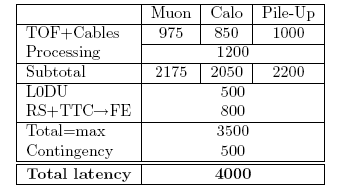
\includegraphics[width=0.55\textwidth]{rysunki/introduction/l0.png}
 \caption{Poszczególne fazy L0. Liczby oznaczają czas wykonania w ns.}
\end{figure}

\noindent
Decyzja L0 oparta jest na odczycie z kalorymetrów elektromagnetycznego (ECal) i hadronowego (HCal), ze stacji mionowych, oraz tzw. systemu Pile-up (PU).
\\\\
System PU kontroluje czy w zderzeniu pęczków mamy tylko jedno zderzenie proton-proton. Jeśli jest ich więcej system ten doprowadza do odrzucania takich zdarzeń. Składa się on z dwóch płytek detektorów krzemowych znajdujących się po przeciwnej stronie punktu zderzenia (rys. 2.2). Szybki algorytm rekonstrukcji pierwotnych wierzchołków oddziaływania służy do wyznaczenia ilości zderzeń proton-proton.
\\
\begin{figure}[!h]
 \centering
 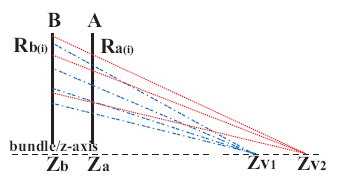
\includegraphics[width=0.5\textwidth]{rysunki/introduction/pileup.png}
 \caption{System Pile-up w przekroju r-z.}
\end{figure}

\noindent
Produkty rozpadu mezonów \textit{B} w związku z dużą masą kwarku \textit{b}, a co za tym idzie dużą masą mezonu zawierają lepton, hadron lub foton charakteryzujący się wysoką energią poprzeczną ($E_T$). Dlatego też decyzja L0 opiera się na rekonstrukcji:
\begin{itemize}
 \item hadronu, elektronu i fotonu o najwyższym $E_T$ w kalorymetrach elektromagnetycznym i hadronowym,
 \item dwóch mionów o najwyższym $E_T$ w każdym z czterech kwadrantów komór mionowych.
\end{itemize}

\noindent
Ponadto zliczana jest ilość naładowanych śladów występujących w zderzeniu. W tym celu wyznaczana jest liczba trafionych cel detektora SPD (Scintilating Pad Detector) umieszczonego tuż przed kalorymetrami. Na podstawie tej informacji odrzucane są przypadki ze zbyt dużą ilością śladów jako zbyt trudne do analizy i pełnej rekonstrukcji. Dla każdego przypadku obliczana jest także całkowita energia poprzeczna zdeponowana w kalorymetrze hadronowym (suma po wszystkich celach HCal) w celu odrzucenia przypadków bez wyraźnego zderzenia proton-proton.
\\\\
Aby pozytywna decyzja L0 została podjęta muszą być spełnione następujące warunki:
\begin{itemize}
 \item tylko jedno zderzenie \textit{pp} w przecięciu pęczków wyznaczone na podstawie informacji z systemu PU, ilość śladów naładowanych obliczona na podstawie sumy po celach SPD musi być mniejsza niż 280, oraz całkowita energia poprzeczna zdeponowana w HCal powyżej 5 GeV,
 \item przynajmniej jeden hadron, elektron, mion lub foton o energii powyżej progu na $E_T$, lub dwa miony o energiach powyżej progu (próg na $E_T$ różni się w zależności od rodzaju i ilości cząstek).
\end{itemize}

\noindent
Wstępna selekcja wykonywana przez L0 odrzuca przypadki z produkcją lekkich kwarków (próg na $E_T$). Jednocześnie rozdziela przypadki ze względu na rodzaj cząstki, która wywołała decyzję (elektron, foton, hadron, mion, $\pi^0$). Tak skonstruowana wstępna selekcja przypadków ułatwia dalszą analizę zdarzenia wykonywaną przez wysoki stopień trygera. Po podjęciu pozytywnej decyzji L0 przypadek jest kierowany na farmę komputerową gdzie wykonany zostanie na nim algorytm HLT.

\subsection{Wysoki poziom trygera - HLT}

HLT, czyli wysoki poziom systemu wyzwalania jest drugą i ostatnią częścią selekcji przypadków przed zapisaniem na nośnik stały z przeznaczeniem do pełnej rekonstrukcji i analizy. Przypadki pojawiają się na wejściu HLT z częstotliwością 1 MHz i analizowane są na farmie komputerowej posiadającej ok. 1800 procesorów. Algorytm HLT dla konkretnego przypadku będzie wykonywany przez jeden procesor, a cały system kontrolowany jest w ramach specjalnego systemu kolejkowania. HLT ma dostęp do danych z całego detektora, jednakże informacje pochodzące z detektorów Czerenkowa mogą być wykorzystane jedynie w jego końcowej fazie przy zredukowanej częstotliwości przypadków. W odróżnieniu od L0, HLT nie ma ustalonego maksymalnego czasu wykonania, jednakże całość algorytmu powinna być wykonana w średnim czasie rzędu kilku milisekund. Średni czas analizy wynika z liczby dostępnych procesorów i ich szybkości.
\\\\
\noindent
Wysoki poziom systemu wyzwalania jest skonstruowany w formie równoległych alei. Celem takiej konstrukcji jest tzw. potwierdzanie - jeżeli L0 dało pozytywną decyzję dla hadronu o wysokim $E_T$, HLT będzie analizował taki przypadek w alei hadronowej. Schemat struktury HLT przedstawia  rysunek 2.3. Zależnie od decyzji L0 przypadek jest kierowany do odpowiedniej alei, gdzie w zależności od wymagań wykorzystuje się różne elementy rekonstrukcji przydatne do selekcji przypadków. Może się zdarzyć, że przypadek otrzyma kilka pozytywnych decyzji L0 np. hadron i elektron, wtedy będzie on analizowany przez wszystkie aleje odpowiadające decyzjom L0. Zysk na czasie spowodowany jest faktem, iż każdy przypadek przechodzi tylko część całego algorytu HLT w zależności od jego wstępnej klasyfikacji przez pierwszy stopień systemu wyzwalania, a rekonstruckja wspólnych obiektów wykonywana jest tylko raz.
\\

\begin{figure}[!h]
 \centering
 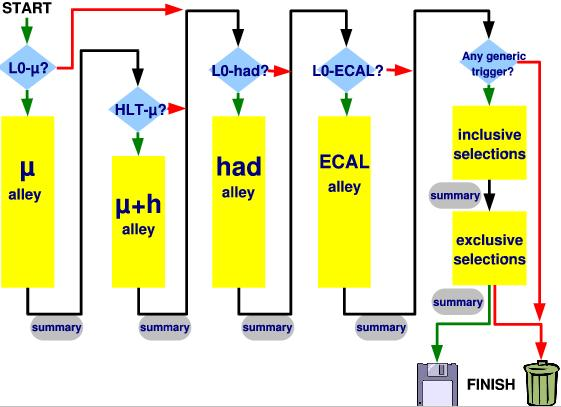
\includegraphics[width=0.8\textwidth]{rysunki/introduction/aleje.jpg}
 \caption{Struktura HLT.}
\end{figure}

\noindent
Celem każdej alei jest selekcja przypadków pod względem konkretnych interesujących nas rozpadów mezonów \textit{B}. Pomimo różnorodności rozpadów mezonów pięknych schemat konstrukcji każdej alei jest podobny (co jest zilustrowane na rys. 2.4).\\

\begin{figure}[!h]
 \centering
 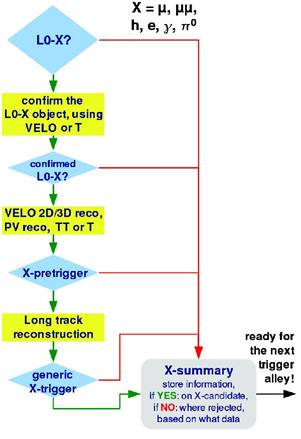
\includegraphics[width=0.4\textwidth]{rysunki/introduction/aleja.jpg}
 \caption{Schemat alei HLT.}
\end{figure}

\noindent
Prostokąty oznaczają elementy rekonstrukcji zaś romby podjętą decyzję trygera. W pierwszej kolejności potwierdzany jest obiekt L0 (elektron, hadron, mion) w oparciu o detektory Velo lub TT. W przypadku fotonowej decyzji L0 nie ma możliwości potwierdzenia fotonu dopasowanym do niego śladem. W następnej kolejności rekonstruowane są trajektorie cząstek w detektorach śladowych, a także wierzchołek pierwotnego oddziaływania. Ze względu na czas życia mezonów \textit{B} ślady produktów ich rozpadu charateryzują się dużym parametrem zderzenia względem pierwotnego wierzchołka zderzenia proton-proton. W tym punkcie mechanizm trygera opiera się na selekcji zdarzenia w przypadku znalezienia śladów dwuwymiarowych, a następnie trójwymiarowych o parametrze zderzenia w odpowiednim przedziale (dla śladów 2D 0.1 - 3 mm, oraz 0.15 - 3 mm dla 3D). Następnie rekonsturowane są długie ślady (przechodzące przez pole magnetyczne magnesu i dające sygnał także w stacjach T - rys 1.1). Poszczególne kroki stosuje się po to by zmniejszać stopniowo częstotliwość przypadków pozostawiając więcej czasu na bardziej wymagającą rekonstrukcję. Przedstawiony schemat jest ogólny, jednakże szczegóły konkretnych alei mogą się różnić. Spowodowane jest to faktem, iż algorytmy konstruowane są pod kierunkiem konkretnych rozpadów mezonów \textit{B} tak, aby uzyskać jak największą wydajność dla interesujących kanałów rozpadu. 
\\\\
\noindent
Celem algorytmów alei jest obniżenie częstotliwości przypadków akceptowanych do ok. 20 kHz łącznie. Kolejna selekcja przypadków odbywa się poprzez inkluzywną i ekskluzywną selekcję (rys. 2.3), której celem jest obniżenie częstotliwości do docelowych 200Hz zdarzeń, które będą zapisane. Ze względu na zredukowaną częstotliwość przychodzenia przypadków po kroku HLT1 wykonywana jest praktycznie pełna rekonstrukcja przypadku, która umożliwia zapisanie ich z docelową częstością 200 Hz. Konstrukcja systemu wyzwalania pozwala na zapisywanie przypadków z częstotliwością 2 kHz, jednakże jedynie 200 Hz pochodzi z ekskluzywnej selekcji rozpadów mezonów \textit{B} (najciekawszych pod względem fizycznym), a pozostałe 1800 Hz pochodzi z innych kontrolnych linii trygera służących do monitorowania poprawności działania eksperymentu.

\section{Aleja elektromagnetyczna wysokiego poziomu systemu wyzwalania}

Zgodnie ze schematem HLT do alei elektromagnetycznej będą trafiać przypadki dla których L0 daje jedną z sygnatur elektromagnetycznych. Należą do nich foton i elektron. Na obecnym etapie eksperymentu nie bierze się pod uwagę trygera dla $\pi^0$.
\\\\
\noindent
W pierwotnej wersji trygera został napisany prototyp algorytmu dla alei elektromagnetycznej HLT, który był punktem wyjścia do budowy bardziej zaawansowanej wersji.
\\\\
\noindent
W pracy opisane zostanie w szczegółach opracowanie algorytmu dla części fotonowej alei elektromagnetycznej dedykowanej rozpadom mezonów \textit{B} zawierających foton (rozdział 3). Do optymalizacji wykorzystano dwa radiacyjne kanały rozpadu, mianowicie $B^{0}_{s}\rightarrow \phi(K^{+}K^{-})\gamma$ oraz $B^{0}_{d}\rightarrow K^{0*}(K^{+}\pi^{-})\gamma$. Działanie algorytmu dla tych kanałów rozpadu jest reprezentatywnym testem dla całej alei fotonowej i jego efektywność dla tych dwóch rozpadów (są to najważniejsze kanały z punktu widzenia analizy fizycznej) jest miernikiem poprawności działania algorytmu dla wszystkich rozpadów fotonowych.
\\\\
\noindent
Celem modyfikacji algorytmu jest osiągnięcie jak najwyższej efektywności dla rozpadów $B^{0}_{s}\rightarrow \phi(K^{+}K^{-}) + \gamma$ oraz $B^{0}_{d}\rightarrow K^{0*}(K^{+}\pi^{-}) + \gamma$ (dalej nazywanych sygnałem). Jednocześnie wymagane jest, aby aleja przepuszczała nie więcej niż 3 kHz przypadków tła (tzw. przypadki \textit{minimum bias}). Na wstępie HLT częstotliwość przychodzenia przypadków wynosi 1 MHz, przy czym przypadki są kierowane do odpowiednich alei zgodnie ze schematem na rys. 2.3, zaś zadaniem alei jest obniżenie częstotliwości do poziomu 20 kHz łącznie. Wartość 3 KHz została przyjęta jako nominalna dla fotonowej części alei elektromagnetycznej. Tłem dla naszego sygnału są wszystkie przypadki zderzenia proton-proton, nie zawierające produkcji pary kwarków $b\bar{b}$ i wpadające do alei elektromagnetycznej.

\chapter{Algorytm systemu wyzwalania dla radiacyjnych rozpadów mezonów B}
\addcontentsline{toc}{chapter}{Algorytm systemu wyzwalania dla radiacyjnych rozpadów mezonów B}
\section{Analiza przypadków w oparciu o symulacje Monte Carlo dla sygnału i tła}

W trakcie przygotowywania eksperymentu LHCb do dyspozycji mamy jedynie przypadki otrzymane z symulacji zderzeń proton-proton i odpowiedzi detektora. W momencie uruchomienia eksperymentu dostępne będą rzeczywiste dane, co może spowodować konieczność dostrojenia algorytmów, jednakże na obecnym etapie korzystamy z symulacji Monte Carlo. Pakiety symulacyjne używane do generacji przypadków (PYTHIA 6.2 [3]) i odpowiedzi detektora (GEANT4 [3]) są narzędziami wielokrotnie sprawdzonymi poprzez porównanie symulacji z rzeczywistymi zdarzeniami. Pozwala to na wiarygodną symulację procesów fizycznych jak i działania detektora podczas opracowywania algorytmu trygera. Należy także dodać, że niektóre efekty są trudne do symulacji np. symulacja szumu elektroniki jest zawsze obarczona znaczną niepewnością.
%\\\\
%\noindent

\subsection{Próbki danych z symulacji Monte Carlo}

Dane dotyczące sygnału dla dwóch kanałów rozpadu mezonów \textit{B}, $B^{0}_{s}\rightarrow \phi\gamma\rightarrow K^+K^-\gamma$ oraz $B^{0}_{d}\rightarrow K^{0*}\gamma\rightarrow K^+\pi^-\gamma$ zostały wyselekcjonowane stosując pełną rekonstrukcję zderzenia (bez użycia trygera). Sygnał był generowany poprzez wymuszenie rozpadu \textit{B} do zadanego kanału w każdym przypadku, natomiast tłem dla sygnału selekcji \textit(off-line) była inkluzywna próbka $b\bar{b}$ gdzie wszystkie produkty rozpadu przynajmniej jednego mezonu \textit{B} emitowane są w obrębie akceptancji detektora. Szczegóły selekcji opisane są w pracy [2]. Ponieważ oba kanały rozpadu są bardzo podobne do siebie pod względem produktów rozpadu, zawierają foton i krótkożyciowy neutralny mezon o masie ok. 1 GeV ($\phi$,$K^{0*}$) rozpadający się na dwa hadrony o przeciwnych znakach ładunku elektrycznego, dlatego też oba kanały można analizować łącznie. Dane zostały wyselekcjonowane tak aby wielkość:
\[
 \xi = \frac{S}{\sqrt{S+T}}
\]
była maksymalna. S - oznacza liczbę przypadków sygnału, T - liczbę przypadków tła. Selekcja przypadków oparta jest na następujących kryteriach:
\begin{itemize}
 \item mezony $B_{d,s}$ są produkowane w obrębie stożka akceptancji detektora LHCb. Kąt rozwarcia stożka wynosi 400 mrad,
 \item sygnałowy foton jest identyfikowany jako klaster w kalorymetrze elektromagnetycznym, nie stowarzyszony z żadnym naładowanym śladem (możliwośc konwersji fotonu na parę elektron-pozyton przed dotarciem do kalorymetrów jest także uwzględniona); jednocześnie z powodu kinematyki dwuciałowego rozpadu mezonu \textit{B} dającej wysokie spektrum energii poprzecznej $E_T$ fotonu, wymagane jest $E_T > 2.8$ GeV, dla redukcji tła pochodzącego od miękkich fotonów z rozpadu $\pi^0$ (dla porównania L0 wymaga klastra fotonowego o $E_T$ powyżej 2.3 GeV, ale są to inne klastry obliczane w oparciu o szybki algorytm stosowany w pierwszym stopniu trygera),
 \item piony oraz kaony naładowane są identyfikowane przy użyciu detektorów RICH1 i RICH2 oraz stowarzyszenia śladu do identyfikowanych cząstek; wykorzystywana jest różnica logarytmicznych prawdopodobieństw dla poszczególnych rodzajów cząstek, np. dla selekcji pionu stosuje się warunek $log\frac{P(\pi)}{P(K)} > -5$, dla selekcji kaonów warunki są różne w zależności od tego czy pochodzą one z rozpadu $\phi$ czy $K^{0*}$,
 \item  w celu identyfikacji parametru zderzenia (Impact Parameter - IP) względem pierwotnego wierzchołka oddziaływania dla dwóch śladów pochodzących od naładowanych hadronów ($K^{+}K^{-}$ oraz $K^{+}\pi^{-}$) obliczany jest współczynnik $\chi^{2} = \left(IP/\sigma_{IP}\right)^{2}$. Ze względu na długi czas życia mezonów \textit{B} produkty ich rozpadów nie celują w wierzchołek pierwotny, dlatego stosuje się dla obu śladów cięcie $\chi^{2}>25$
\end{itemize}
\noindent
Szczegóły pełnej rekonstrukcji i selekcji radiacyjnych rozpadów mezonów \textit{B} mogą być przydatne w konstrukcji trygera, ponieważ można próbować stosować podobne cięcia już na etapie systemu wyzwalania. Jednakże informacje dostępne do podjęcia decyzji podczas wykonywania algorytmu alei są ograniczone np. informacja z detektorów Czerenkowa jest niedostępna, parametr zderzenia śladu jest wyznaczony bez błędu, klastry elektromagnetyczne są wyznaczane innym algorytmem itd.
\\\\
\noindent
Do analizy opisywanej w pracy mieliśmy do dyspozycji próbkę danych sygnałowych zawierającą 1291 wyselekcjonowanych przypadków rozpadu $B_s\rightarrow \phi\gamma$ oraz 2245 przypadków rozpadu $B_d\rightarrow K^{0*}\gamma$, co daje łączną liczbę 3536 przypadków sygnałowych (dane dla obu kanałów możemy analizować łącznie, co daje nam większą statystykę). 
\\\\
\noindent
Przypadki te wyselekcjonowane zostały przez pełną rekonstrukcję odczytu detektora LHCb, jednakże spośród tych przypadków jedynie 2466 zdarzeń (69.7\%) otrzymuje pozytywną decyzję L0 z dowolną sygnaturą (najczęściej foton, elektron, $\pi^0$). Oznacza to, że 30\% przypadków jest odrzucane na podstawie globalnych informacji o przypadku tj. zrekonstruowana w trygerze ilość zderzeń proton-proton w przypadku lub ilość naładowanych śladów. Ponadto do alei elektromagnetycznej z sygnaturą fotonową (pozytywna decyzja fotonowa L0) wpada 1231 przypadków (50\% przypadków z pozytywną globalną decyzją L0, 34,8\% spośród wszystkich przypadków sygnału). L0 jest trygerem sprzętowym i jego efektywność dla interesujących nas przypadków rozpadu mezonów \textit{B} może być daleka od stu procent.
\\\\
\noindent
Jednym z powodów obserwowanej efektywności L0 może być konwersja sygnałowego fotonu na parę elektron-pozyton przed dotarciem do kalorymetru elektromagnetycznego. Ilość materiału konstrukcyjnego detektorów w długościach radiacyjnych $X_0$ przedstawia rysunek 3.1 [4]. 

\begin{figure}[!h]
 \centering
 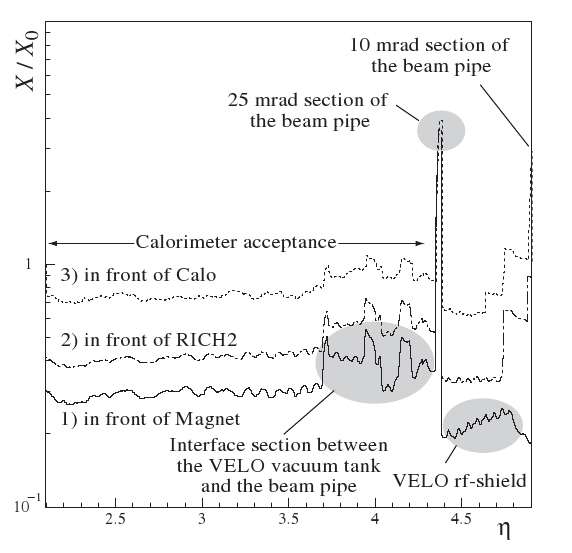
\includegraphics[width=0.5\textwidth]{rysunki/radiationl.png}
 \caption{Materiał widziany przez neutralną cząstkę od punktu zderzenia w funkcji pseudorapidity dla trzech różnych pozycji wzdłuż osi detektora, uśredniona po kącie azymutalnym.}
\end{figure}

\noindent
Interesująca jest dla nas trzecia, najwyższa linia ilości materiału przed kalorymetrem elektromagnetycznym. Przed kalorymetrem znajdują się detektory śladowe VELO, TT oraz stacje T1-T3, dwa detektory Czerenkowa RICH1 i RICH2 i jedna stacja mionowa M1 (rys. 1.1). Dają one około jedną długość radiacyjną materiału co może powodować konwersję części sygnałowych fotonów na pary $e^{+}e^{-}$ przed dotarciem do kalorymetrów. W takim przypadku klastry elektromagnetyczne od elektronu i pozytonu w kalorymetrze nie dają sygnatury fotonowej (ze względu na korelacje z naładowanym śladem) co przekłada się na obniżenie efektywności L0 dla rozpadów fotonowych.
\\\\
\noindent
W celu sprawdzenia tego efektu można znaleźć, na podstawie informacji z symulacji Monte Carlo (MC), w którym miejscu na osi detektora następuje konwersja sygnałowego fotonu. Rozkład tych położeń na osi $\hat{z}$ detektora przedstawia rysunek 3.2.

\begin{figure}[!h]
 \centering
 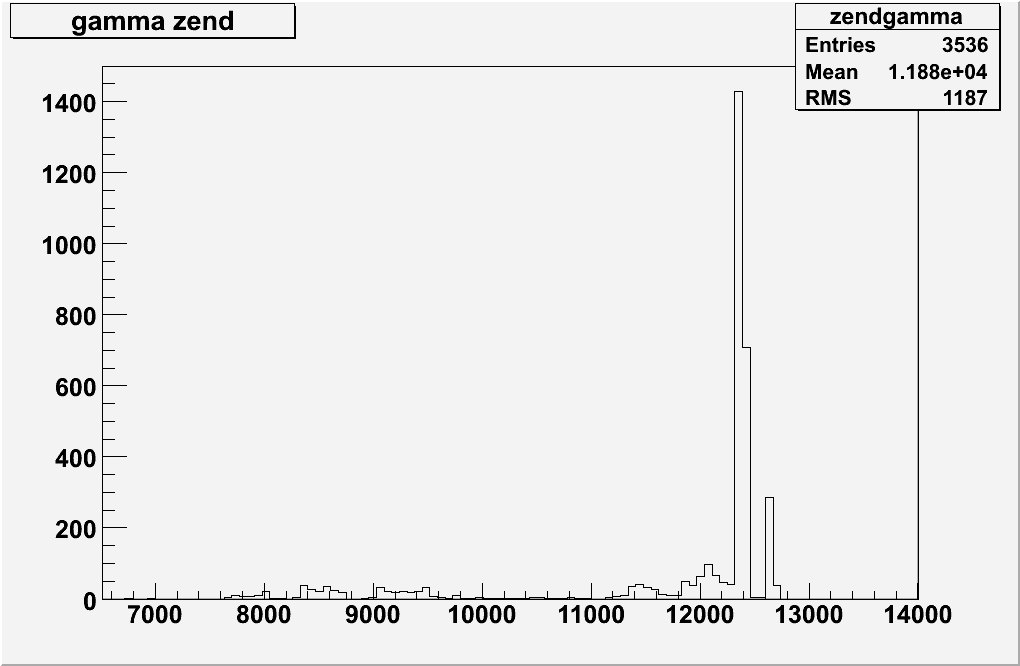
\includegraphics[width=0.6\textwidth]{rysunki/zend.png}
 \caption{Punkt na osi $\hat{z}$ detektora (w mm) w którym sygnałowy foton ulega konwersji.}
\end{figure}
 
\noindent
Około jedna długość radiacyjna materiału wpływa znacząco na czystość próbki fotonów co widać na rysunku 3.2. 30\% fotonów nie dolatuje do kalorymetru (1056 przypadków). Natomiast widoczna jest wyraźna kumulacja pochodząca od fotonów, które konwertują w materiale detektora PS\footnote{PreShower (PS) - detektor ten jest warstwą 2.5 długości radiacyjnych ołowiu umieszczoną przed kalorymetrem elektromagnetycznym, służy on rozróżnianiu pomiędzy cząstką naładowaną a neutralną (głównie elektronem a fotonem). Obie cząstki zaczynają tworzyć kaskadę elektromagnetyczną w płytce ołowiu, jednakże elektron daje sygnał bezpośrednio przed PS i bezpośrednio za nim, w momencie gdy foton daje sygnał tylko za PS.} (z=12300 mm), a także pozostałe fotony, które konwertują dopiero w materiale kalorymetru elektromagnetycznego. Tak więc tylko fotony konwertujące w PS lub dalej mają szansę na uzyskanie akceptacji przez L0 jako foton. Efekt ten częściowo wyjaśnia niską wydajność fotonową L0. Należy jednocześnie pamiętać, iż rekonstrukcja klastrów elektromagnetycznych na poziomie L0 jest uproszczona [3] i może spowodować dodatkowe obniżenie wydajności pierwszego stopnia trygera dla fotonów. Mechanizm tworzenia klastrów L0\footnote{Klastry dla pierwszego stopnia trygera są tworzone w oparciu o zbiorczą informację z 4 sąsiednich cel kalorymetru elektromagnetycznego} może błednie zidentyfikować tylko część klastra fotonowego, co przekłada się na niepoprawny pomiar energii poprzecznej fotonu (L0 wymaga $E_T$ klastra fotonowego powyżej 2.3 GeV). Algorytm alei fotonowej HLT ma do dyspozycji jedynie pozostałe 34.8\% wszystkich przypadków sygnałowych wyselekcjonowanych przez pełną rekonstrukcję, na podstawie których będzie w dalszej części pracy opisana konstrukcja algorytmu. W stosunku do tej liczby będzie też liczona efektywność działania alei fotonowej.
\\\\
\noindent
Pozostała część przypadków sygnałowych, które przechodzą przez L0, otrzymuje inną niż fotonową sygnaturę, głównie elektron lub $\pi^0$. Jednakże w takich przypadkach istnieje prawdopodobieństwo zadziałania trygera na cząstkach nie pochodzących od sygnałowego mezonu \textit{B}, co znacznie utrudnia późniejszą analizę przypadku. Podczas konstrukcji algorytmu należy zwrócić uwagę nie tylko na efektywność działania, ale także i na to, aby decyzję podejmować w oparciu o cząstki i sygnatury fizyczne sygnałowych rozpadów.
\\\\
\noindent
Przypadki tła są generowane jako zderzenia proton-proton uwzględniając twarde procesy QCD, pojedyncze i podwójne procesy dyfrakcyjne oraz rozpraszanie elastyczne. Dla celów projektowania algorytmu do dyspozycji mieliśmy łącznie 38304 przypadki tła zaakceptowane przez pierwszy stopień systemu wyzwalania L0. Do alei fotonowej po zaakceptowaniu przez L0 jako foton wpada 4592 przypadków (12\%), jednakże w przypadku tła, ze względu na fakt iż w eksperymencie LHCb przypadki sygnałowe stanowią znikomą część wszystkich zdarzeń, wygodniej jest mówić o częstotliwości przychodzenia przypadków. Na wstępie części alei fotonowej wynosi ona 120 kHz (z taką częstotliwością będzie uruchamiana aleja fotonowa). Liczba ta oznacza, iż zadaniem alei fotonowej jest przynajmniej 40-krotne obniżenie częstotliwości dla tła (3 kHz to maksymalna dozwolona częstotliwość wynikająca z konstrukcji HLT) przy możliwie jak największej wydajności dla przypadków sygnałowych.
\\\\
\noindent
Do analizy danych w pracy wykorzystano pakiet DaVinci v19r8 z oficjalnego oprogramowania eksperymentu LHCb (służy do fizycznej analizy przypadków), pakiet HLT v1r11 (odpowiadający za wykonanie algorytu wysokiego stopnia systemu wyzwalania), a także pakiet ROOT wersja 5.14. Przy opracowywaniu algorytmu separacji $\pi^0$/foton (paragraf 3.2.1) wykorzystano pakiet do wielowymiarowej analizy danych w oparciu o sieci neuronowe TMVA (Toolkit for Multivariate Data Analysis with ROOT)[6].

\section{Opracowanie algorytmu i efektywność działania}
Oryginalna wersja alei fotonowej odzwierciedla historyczną strukturę pochodzącą z trzystopniowego systemu wyzwalania. Mechanizm odrzucania przypadków zakłada następujące kryteria (podano sekwencję cięć trygera na podstawie oprogramowania HLT v1r11):
\begin{itemize}
 \item[-] $E_T$ fotonowego klastra z L0 powyżej 2,9 GeV,
 \item[-] przynajmniej jeden ślad o dwuwymiarowym parametrze zderzenia (r-z) w granicach 0.1-3 mm,
 \item[-] spośród śladów wybranych na podstawie dwuwymiarowego parametru zderzenia, przynajmniej jeden ślad o trójwymiarowym parametrze zderzenia w granicach 0.15-3 mm,
 \item[-] pęd poprzeczny wybranego wcześniej śladu powyżej 1,3 GeV. 
\end{itemize}
\noindent
Zastosowanie tego algorytmu przy obecnej dwustopniowej konstrukcji trygera daje jedynie 56\% efektywności dla sygnału (efektywność ta jest liczona względem przypadków sygnału wpadających do alei fotonowej), przy częstotliwości akceptacji dla tła na poziomie 8 kHz. Algorytm ten przy stosunkowo niskiej wydajności dla sygnału przepuszcza ponad dwa razy więcej tła niż jest to dozwolone dla alei, tak więc wymaga on powtórnego sprawdzenia i optymalizacji. Szczegóły analizy i optymalizacji algorytmu alei elektromagnetycznej będą opisane w kolejnych podrozdziałach. 

\subsection{Analiza klastrów elektromagnetycznych}
Jedną za najważniejszych sygnatur sygnałowych kanałów rozpadu jest wysokoenergetyczny foton. Klaster fotonowy powinien znajdować się w obrębie kalorymetru elektromagnetycznego i jak wiemy z pełnej rekonstrukcji posiadać energię poprzeczną powyżej 2.8 GeV. Na tym poziomie analizy rozpatrywane są klastry w kalorymetrze elektromagnetycznym tworzone już dla pierwszego stopnia trygera. Są one dostępne także dla HLT (znajdują się w zbiorze o nazwie L0CaloCandidates). Przypadki sygnałowe, które wpadają do alei fotonowej zawierają niewielką ilość (3,3\%) fotonów konwertujących przed ECal, tak więc w większości zdarzeń powinien znajdować się wysokoenergetyczny fotonowy klaster pochodzący wprost z rozpadu mezonu \textit{B}. W celu sprawdzenia klastrów fotonowych emulowane jest działanie L0 i sprawdzane ile i jakiego rodzaju (typ cząstki) klastrów znajduje się w zdarzeniach sygnału i tła (emulacja L0 wymaga $\mathrm{E_T>2.3}$ GeV oraz odpowiedniego typu klastra w kalorymetrze elektromagnetycznym). Okazuje się, że w dużej większości zdarzeń w ECal znajduje się tylko jeden klaster odpowiadający wymogom L0 dla fotonu zarówno dla sygnału (90,7\%) jak i dla tła (93\%), w pozostałych przypadkach znajdują się 2 klastry. Ponadto wykorzystano asocjację klastrów elektromagnetycznych do cząstek Monte Carlo aby zobaczyć jakie cząstki w przypadkach tła dają pozytywną decyzję fotonową L0. Służy to także sprawdzeniu czy pozytywną decyzję L0 daje sygnałowy foton. Wnioski z obserwacji są następujące:
\begin{itemize}
 \item dla danych sygnałowych w 96\% przypadków L0 jest wyzwalany na klastrze fotonowym pochodzącym bezpośrednio z rozpadu \textit{B} (pozostałe przypadki akceptowane są dzięki cząstkom niesygnałowym). Spośród wszystkich klastrów w ECal 93\% stanowią fotony, występuje też mała domieszka klastrów pochodzących od $\pi^0$, które także spełniają warunki fotonu dla L0 (6,6\%),
 \item w przypadkach tła największą ilość klastrów stanowią $\pi^0$, aż 77\%, następnie fotony 15\%, piony naładowane 4\%, a resztę stanowią domieszki innych cząstek.
\end{itemize}
 
\noindent
Fotony w przypadkach \textit{minimum bias} stanowią nieredukowalne tło spełniające wszystkie warunki sygnałowych fotonów na tym etapie selekcji (wysoka energia poprzeczna, brak stowarzyszonego śladu). Tak więc rozważając klastry elektromagnetyczne jakie tworzą się w ECal, największe tło pochodzi od mezonów $\pi^0$. Nie ma także sensu stosować asocjacji śladu do powyższych klastrów celem odrzucania klastrów dla których znaleziono ślad, ponieważ ogromna większość klastrów zarówno dla sygnału jak i tła pochodzi od cząstek neutralnych. W poprzedniej realizacji trygera nie stosowano algorytmów na separację pomiędzy $\pi^0$ a fotonem, jednakże powyższa analiza wskazuje, iż taka separacja na poziomie trygera może znacząco obniżyć częstotliwość przypadków tła. Algorytm separacji $\pi^0$/foton oraz analiza jego działania na poziomie HLT zostanie opisana w kolejnym podrozdziale (3.2.2).
\\\\
\noindent
Ponieważ próg na $E_T$ dla klastrów fotonowych dla pierwszego stopnia trygera wynosi 2,3 GeV, a dane do których należy dostosować tryger zawierają fotony o energii poprzecznej powyżej 2,8 GeV, można podnieść ten próg bez dużych strat na sygnale. Tabela 3.1 pokazuje jak zmieniają się efektywności dla sygnału i tła gdyby stosować cięcie dla L0 z wyższym progiem (takie podejście zaprezentowane było we wcześniejszym algorytmie alei fotonowej dla HLT). Teraz jak i później efektywność tła będzie podawana w stosunku do poziomu tła na początku alei fotonowej.
\begin{table}[!h]
 \centering
 \begin{tabular}{|c|c|c|}
  \hline
  $E_T$ [GeV] & Efektywność sygnału & Efektywność tła \\
  \hline 
  2,3 & 100\% & 100\% \\
  \hline
  2,6 & 97,8\% & 70,5\% \\
  \hline
  2,7 & 96,4\% & 63,0\% \\
  \hline
  2,8 & 93,6\% & 56,3\% \\
  \hline
  2,9 & 89,1\% & 50,5\% \\
  \hline
 \end{tabular}
 \caption{Efektywność w zależności od cięcia na $E_T$ klastra fotonowego.}
\end{table}
\\
\noindent
Mimo iż dane sygnałowe zostały wyselekcjonowane z zastosowaniem cięcia na energię poprzeczną klastra fotonowego powyżej 2,8 GeV, zastosowane w trygerze tak wysokie cięcie odrzuca jeszcze część sygnału. Dzieje się tak dlatego, gdyż pomiar energii poprzecznej w trygerze jest uproszczony i może nie zgadzać się dokładnie z rzeczywistą energią fotonowego klastra. Na podstawie tabeli 3.1 widać że cięcie na $E_T$ w regionie 2,6-2,7 GeV jest sensowne do rozważenia w algorytmie alei fotonowej. Opracowanie nowej wersji sekwencji cięć trygera HLT dla alei będzie opisane w rozdziale 3.3

\subsection{Separacja $\pi^0$/foton}

Idea separacji $\pi^0$/foton w eksperymencie LHCb za pomocą szybkiej rekonstrukcji klastrów w ECal została przedstawiona w prezentacji [5]. Separacja ta opiera się na różnicy w kształcie kaskad elektromagnetycznych tworzonych w kalorymetrach dla fotonów i neutralnych pionów. Z uwagi na fakt, iż wysokoenergetyczne $\pi^0$ rozpadające się w niemalże stu procentach na dwa lecące w niewielkiej odległości od siebie fotony istnieje duże prawdopodobieństwo, że fotony te utworzą jeden wspólny klaster w kalorymetrze. Dlatego też taki typ $\pi^0$ określa się mianem połączone (z angielskiego $merged$). Klaster elektromagnetyczny pochodzący od $merged-\pi^0$  charakteryzuje się innym kształtem poprzecznym niż ma to miejsce dla pojedynczego fotonu.
\\\\
\noindent
W pracy [5] do separacji pomiędzy klastrami pojedynczych fotonów a klastrami pochodzącymi od $merged-\pi^0$ wykorzystano pełną rekonstrukcję klastrów w kalorymetrze elektromagnetycznym. Do rozróżnienia pomiędzy rodzajami klastrów użyto zmiennych opisujących kształt kaskad elektromagnetycznych. Zmienne te obliczane są w oparciu o rozkład energii zmierzony w poszczególnych celach kalorymetru należących do danego klastra. W szczególności wzięto pod uwagę następujące zmienne:
\[
 s_{xx}=\frac{\sum_i \epsilon_i \cdot (x_i - \bar{x})^2}{\sum_i \epsilon_i},
 \hspace{15pt}
 s_{xy}=\frac{\sum_i \epsilon_i \cdot (x_i - \bar{x})\cdot (y_i - \bar{y})}{\sum_i \epsilon_i},
 \hspace{15pt}
 \bar{x}=\frac{\sum_i \epsilon_i \cdot x_i}{\sum_i \epsilon_i}
\]
gdzie $s$ jest dwuwymiarową macierzą kowariancji ważoną energią, $x_i$ i $y_i$ oznaczają położenie celi kalorymetru w płaszczyźnie x-y, $\epsilon_i$ zdeponowaną energię w celi $i$, a suma odbywa się po wszystkich celach ECal przypisanych do danego klastra. 
\\\\
\noindent
Zmienne charakterystyczne dla klastrów wybrano tak aby odzwierciedlały cechy kaskady. Schematyczny przekrój klastra przedstawia rysunek 3.3. Same zmienne obliczane są według poniższych wzorów:

\begin{itemize}
 \item $f_{r^2}=<r^2>=s_{xx}+s_{yy}$ \normalsize{ - określa rozciągłość kaskady w płaszczyźnie x-y}, 
 \item $f_{asym}=s_{xy}/\sqrt{s_{xx}\cdot s_{yy}}$ \normalsize{ jest współczynnikiem asymetrii},
 \item $f_{r^2r^4}=(<r^4> - <r^2>^2)/<r^4>$ \normalsize{ - określa stosunek energii zdeponowanej w środku klastra w odniesieniu do energii zdeponowanej na jego obrzeżach},
 \item $f_{\kappa}=\sqrt{1-4\cdot \frac{s_{xx}\cdot s_{yy} - s_{xy}^{2}}{(s_{xx} + s_{yy})^2}}$ 
\normalsize{ - współczynnik ten określa stosunek długości osi głównych elipsy klastra}. 
\end{itemize}

\begin{figure}[!h]
 \centering
 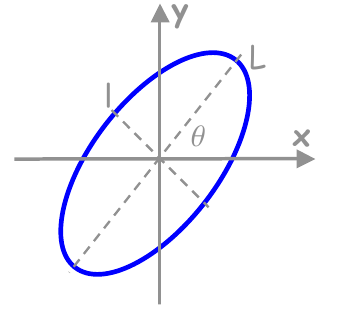
\includegraphics[width=0.4\textwidth]{rysunki/shape.png}
 \caption{Eliptyczny kształt kaskady w kalorymetrze elektromagnetycznym.}
\end{figure}

\noindent
Parametry te zostały dobrane tak, aby wiarygodnie odzwierciedlać kształt kaskady w stosunku do rozkładu zdeponowanej energii w obrębie klastra, co ma kluczowe znaczenie w celu rozróżnienia klastrów pochodzących od pojedynczego fotonu i klastrów pochodzących od $merged-\pi^0$. W pracy [5] separacji dokonywano pomiędzy fotonami i $merged-\pi^0$ pochodzącymi bezpośrednio od sygnałowych mezonów \textit{B}, jednakże problem w przypadku odrzucania klastrów od $\pi^0$ z tła jest analogiczny (cząstki z tła nie są tak dobrze wyselekcjonowane).
\\\\
\noindent
Aby dla klastrów o pozytywnej fotonowej decyzji L0 obliczyć wyżej wymienione parametry kaskady należy skorzystać z pełnej rekonstrukcji klastrów w ECal. Klastry dostępne dla pierwszego stopnia trygera nie mają tak zaawansowanych informacji, jednakże w fazie HLT istnieje możliwość pełnej rekonstrukcji klastrów w kalorymetrze. Z uwagi na to, że dla klastrów o sygnaturze fotonowej z L0 zastosowano cięcie na $\mathrm{E_T>2.3}$ GeV pełna rekonstrukcja klastrów mieści się w ograniczeniach czasowych HLT i można wykonać obliczenie zmiennych kształtu w algorytmie trygera.
\\\\
\noindent
Ponieważ dla każdego klastra posiadamy informację o jego kształcie i energii zdecydowaliśmy się użyć do separacji wielowymiarowej analizy z użyciem pakietu TMVA. Pakiet ten jest kompatybilny z ROOT-em i umożliwia analizę danych pod kątem separacji sygnału od tła stosując różne metody oparte m.in. o sieci neuronowe. Dla celów trygera wymagane jest aby algorytm rozróżniający klastry (klasyfikator) był możliwie najprostszy (zawierał możliwie jak najmniejszą liczbę parametrów) z uwagi na konieczność wykonania algorytmu na każdym klastrze (1 lub 2 w przypadku). Metody wielowymiarowej analizy danych z użyciem pakietu TMVA oraz zasady ich działania są w szczegółach opisane w pracy [6]. 
\\\\
\noindent
Z uwagi na konstrukcję kalorymetru elektromagnetycznego LHCb, parametry do separacji należy dobrać oddzielnie dla wszystkich obszarów ECal różniących się wielkością cel. Pierwszy obszar tworzą kwadratowe cele o bokach o długości 20,2 mm (obszar najbliżej rury akceleratora), dla drugiego obszaru długość boku to 40,4 mm, dla trzeciego 60,6 mm. Dane do separacji zostały przygotowane w następujący sposób:
\begin{itemize}
 \item[-] dla sygnału przygotowano zrekonstruowane klastry pochodzące od sygnałowych fotonów (łącznie ok. 1200 przypadków),
 \item[-] dla tła przygotowano zrekonstruowane klastry pochodzące od $\pi^0$ wymagając aby oba fotony utworzyły jeden klaster w kalorymetrze (łącznie ok. 1400 przypadków). 
\end{itemize}
\noindent
W obu przypadkach wybrano tylko takie klastry, które będą analizowane przez aleję fotonową. Ze względu na konieczność przeprowadzenia analizy oddzielnie dla trzech obszarów kalorymetru, ilość przypadków jest niewielka co może wpłynąć znacząco na wyniki. Do analizy wykorzystaliśmy zmienne kształtu oraz energię całkowitą klastrów. Rysunek 3.4 przedstawia rozkłady tych zmiennych dla danych sygnału i tła z jednego obszaru ECal. \\
\begin{figure}[!h]
 \centering
 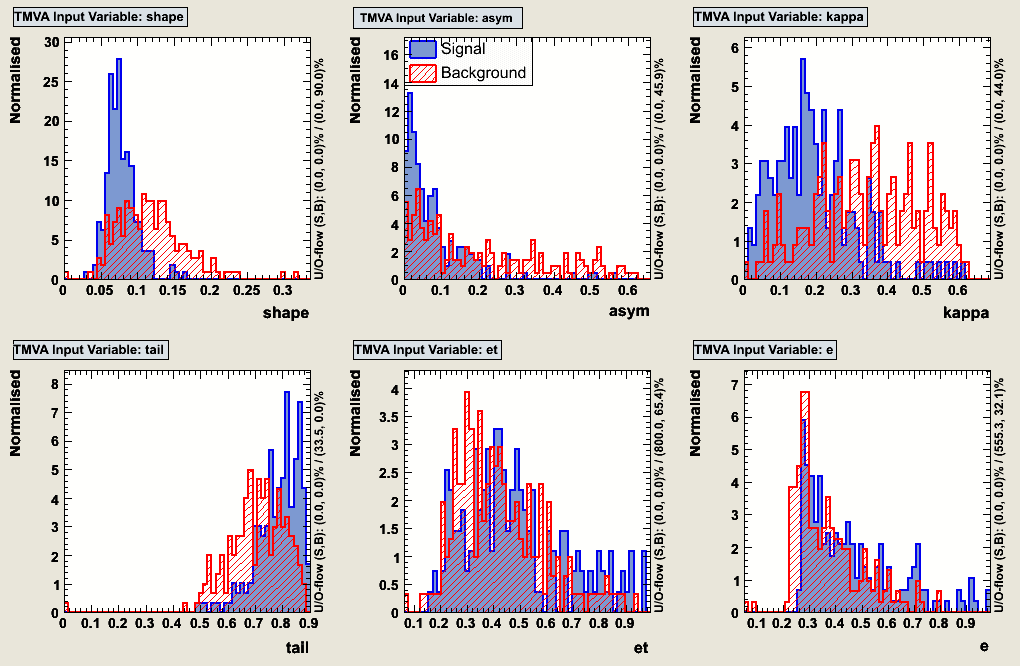
\includegraphics[width=0.9\textwidth]{rysunki/tmva/vars.png}
 \caption{Rozkłady zmiennych kształtu i energii sygnałowych fotonów i $merged-\pi^0$.}
\end{figure}

\noindent
Z rysunku 3.4 widzimy, że rozkłady zmiennych dla sygnału i tła różnią się, ale żaden z nich nie pozwala na dokładną separację. Zastosowanie pakietu do wielowymiarowej analizy pozwala na uwzględnienie korelacji pomiędzy zmiennymi. Dzięki temu efektywność algorytmu jest większa niż w przypadku stosowania niezależnych cięć dla każdego rozkładu z osobna. Rysunek 3.5 przedstawia efektywność działania otrzymanych z analizy klasyfikatorów dla dwóch metod, metody Fishera i SVM (Support Vector Method).\\
\begin{figure}[!h]
 \centering
 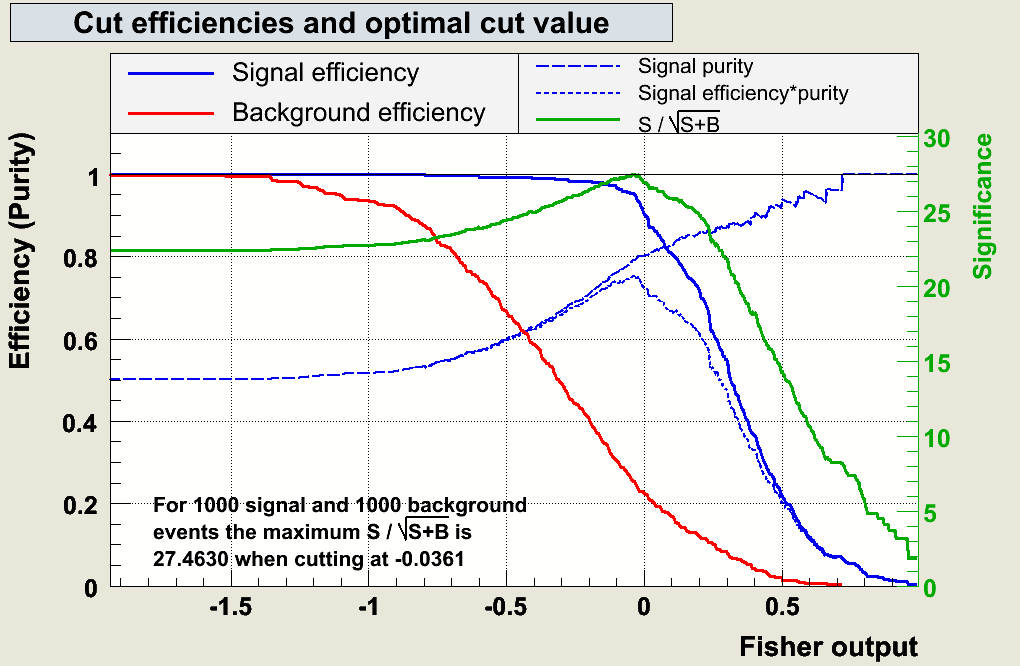
\includegraphics[width=0.49\textwidth]{rysunki/tmva/effFisher.png}
 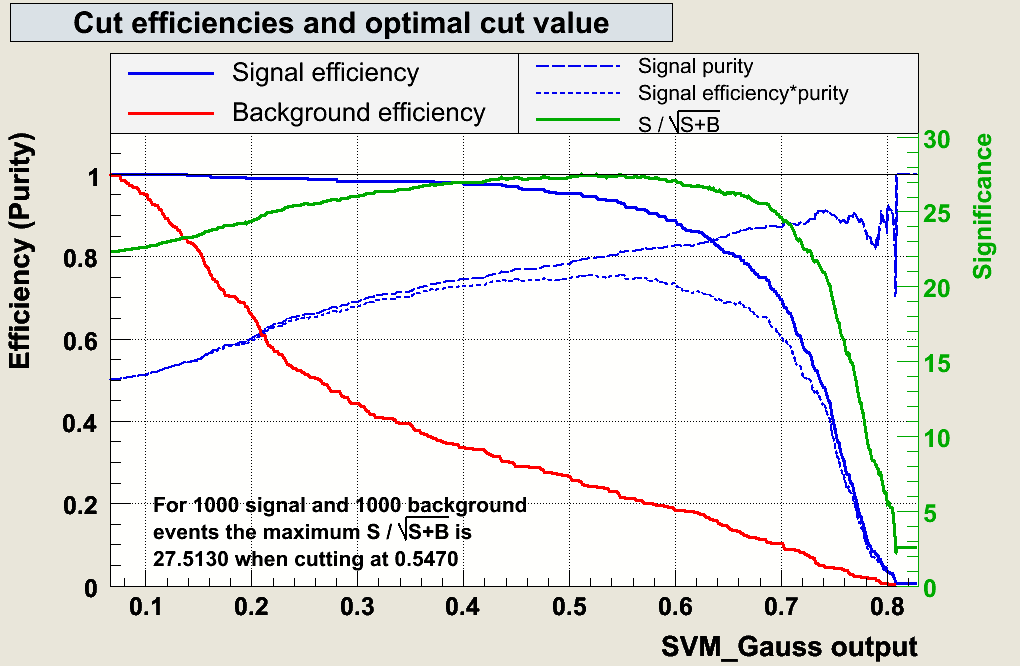
\includegraphics[width=0.49\textwidth]{rysunki/tmva/effSVM.png}
 \caption{Efektywność działania klasyfikatorów dla metody SVM oraz metody Fishera. Linia niebieska reprezentuje efektywność dla klastrów od sygnałowych fotonów w zależności od cięcia. Linia czerwona oznacza analogiczną efektywność dla klastrów od $merged-\pi^0$. Linia zielona przedstawia stosunek efektywności $S/\sqrt{S+B}$.}
\end{figure}

\noindent
Na podstawie rysunku 3.5 możemy stwierdzić, że przy wydajności dla sygnałowych fotonów ok. 90\% tło pochodzące od $merged-\pi^0$ można zredukować pięciokrotnie do poziomu ok. 20\%. Do podjęcia decyzji tworzony jest klasyfikator dla którego w algorytmie możemy wykonać już standardowe cięcie. Wykres dla przykładowego klasyfikatora omawianej separacji przedstawia rysunek 3.6 \\
\begin{figure}[!h]
 \centering
 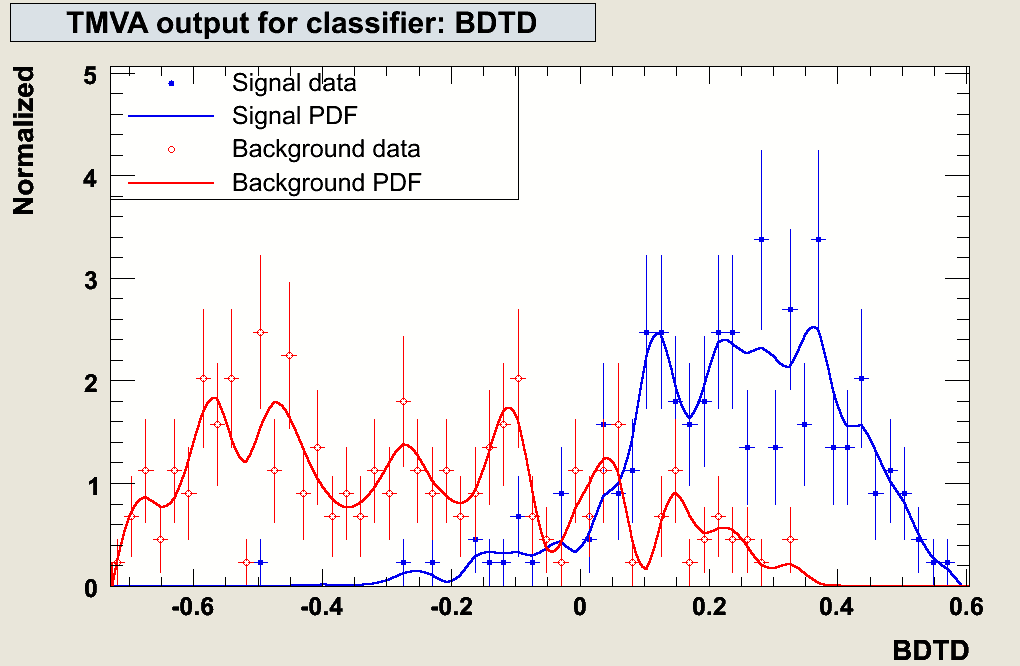
\includegraphics[width=0.5\textwidth]{rysunki/tmva/classifierBDTD.png}
 \caption{Przykładowy klasyfikator dla metody BDTD.}
\end{figure}

\noindent
Wykres klasyfikatora (rys. 3.6) jest nieco poszarpany ze względu na niską statystykę, jednakże wyraźny jest obszar dla którego za pomocą klasyfikatora możemy odrzucić sporą część tła. Dla celów trygera powinniśmy się starać utrzymać efektywność dla sygnału na wysokim poziomie (ok. 90\%) co jednak, według wykresów na rysunku 3.5, pozostawia około 1/5 tła pochodzącego od $merged-\pi^0$.
\\\\
\noindent
Większość metod dostępnych do testowania w pakiecie TMVA daje dla naszych danych podobne efektywności, dlatego też wybrano metodę oraz klasyfikator którego użycie w algorytmie alei jest najprostsze i zawiera możliwie jak najmniejszą liczbę parametrów, jaką jest metoda Fishera. Jej zasada działania została opisana w dodatku A. Metoda Fishera została wprowadzona do emulacji alei fotonowej HLT, którą utworzyliśmy dla celów testowania algorytmu.
\\\\
\noindent
Opisane powyżej wyniki separacji otrzymane zostały dla pojedynczych klastrów. Tak przygotowany algorytm zastosowany został dla wszystkich klastrów fotonowych w przypadku, które powodują pozytywną decyzje fotonową trygera L0. Optymalny punkt pracy pozwolił na maksymalną redukcję klastrów pochodzących od $merged-\pi^0$ przy zachowaniu 90\% efektywności sygnałowej. Dla przypadków tła otrzymana efektywność działania separacji wynosi ok. 50\% (dla pojedynczych klastrów $merged-\pi^0$ wynosi ona 20-25\% w zależności od regionu ECal). Algorytm separacji ma szansę działać efektywnie jedynie dla klastrów pochodzących od cząstek $merged-\pi^0$. Klastry fotonowe, stanowiące 15\% klastrów tła, spełniają dokładnie takie same warunki jak klastry od fotonów pochodzących z rozpadów mezonów \textit{B} na tym etapie selekcji. Dlatego separacja ich nie odrzuca. Wytłumaczeniem efektu słabszego odrzucania tła od klastrów $\pi^0$ jest fakt, iż spośród cząstek $\pi^0$ (tworzą one 77\% klastrów tła dla alei) jedynie 36\% stanowią te dla których oba fotony tworzą jeden wspólny klaster w kalorymetrze. Z tego powodu pozostała część klastrów pochodzących od $\pi^0$ zawiera tylko jeden foton (jeśli kąt rozlotu fotonów jest znaczny, to na poziomie kalorymetru są one na tyle daleko, że tworzą osobne klastry), który także odpowiada wszystkim warunkom sygnałowego fotonu. Rysunek 3.7 pokazuje jak blisko siebie na poziomie kalorymetru elektromagnetycznego znajdują się fotony pochodzące od $\pi^0$ dla rozważanych do odrzucenia klastrów tła. Jeśli fotony znajdują się w odległości od siebie większej niż około 10 cm (w zależności od regionu kalorymetru i energii $\pi^0$) to zostaną dla nich utworzone dwa osobne klastry, z których jeden bądź oba wpadają do alei już jako pojedyncze klastry fotonowe. Należy jednocześnie pamiętać, że klasyfikator wyznaczany jest dla każdego klastra elektromagnetycznego, który spełnia warunki fotonowe dla L0 i wpada do rozważanej alei HLT. W przypadkach zarówno sygnałowych jak i tła znajdują się od jednego do dwóch takich klastrów na przypadek, co może spowodować dodatkowe obniżenie wydajności dla całych przypadków (wystarczy aby tylko jeden spośród klastrów spełnił warunki klasyfikatora).
\begin{figure}[!h]
 \centering
 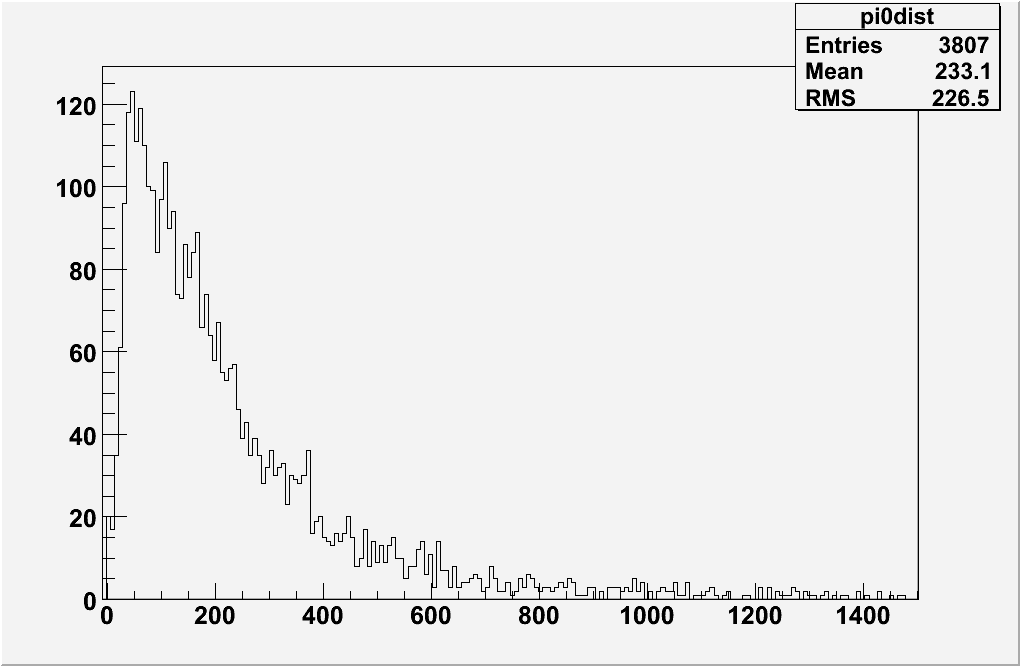
\includegraphics[width=0.6\textwidth]{rysunki/pi0dist.png}
 \caption{Odległość fotonów (w mm) pochodzących od $\pi^0$ na poziomie ECal.}
\end{figure}
\\\\
\noindent 
Analiza powyższa oznacza, że na poziomie klastrów w ECal jedynie 28\% klastrów tła pochodzi od połączonych fotonów z $merged-\pi^0$, zaś tło od klastrów pojedynczych fotonów jest znaczne, przewyższa 65\%. Uzyskanie redukcji tła o połowę z użyciem wielowymiarowej analizy i separacji $merged-\pi^0$/foton jest optymalnym rezultatem. Tabela 3.2 przedstawia efektywności dla sygnału i tła dla algorytmu separacji w trzech regionach ECal.
\begin{table}[!h]
\centering
 \begin{tabular}{|c|c|c|c|}
  \hline
  Region ECal & Wielkość celi & Efektywność sygnału & Efektywność tła \\
  \hline
  I  & 20,2 mm & 89,4\% & 47\% \\
  \hline
  II & 40,4 mm & 88,9\% & 56\% \\
  \hline
  III & 60,6 mm & 85,5\% & 47,4\% \\
  \hline
 \end{tabular}
 \caption{Efektywności dla przypadków sygnału i tła po zastosowaniu algorytmu separacji $merged-\pi^0$/foton dla trzech regionów ECal.}
\end{table}
\\
\noindent
Powyższa analiza ilustruje trudność w separacji sygnałowego fotonu od tła z wykorzystaniem kalorymetru elektromagnetycznego. Sygnałowe fotony w kalorymetrze LHCb obarczone są dużym tłem od klastrów fotonowych z przypadków \textit{minimum bias}. Pochodzą one zarówno od pojedynczych fotonów jak i od neutralnych pionów. Z tego względu, pomimo skutecznej metody na separację pomiędzy klastrami pochodzącymi od $merged-\pi^0$ a klastrami fotonowymi, dla trygera otrzymujemy redukcję tła jedynie o połowę. 
\\\\
\noindent
Dalszą redukcję można uzyskać poprzez podniesienie progu na $E_T$ klastra do 2,7 GeV. Wraz z separacją $merged-\pi^0$/foton pozwala to uzyskać ponad 3-krotne obniżenie poziomu tła, przy blisko 90\% efektywności sygnału. Należy pamiętać, że celem algorytmu alei jest obniżenie tła o czynnik 40, a analiza w oparciu o informacje z kalorymetru elektromagnetycznego jest szybka i wykonywana zawsze na początku sekwencji alei, tak więc może być przydatna do docelowej konstrukcji algorytmu. Wnioski po zastosowaniu cięcia na $E_T$ oraz separacji można przedstawić następująco:
\begin{itemize}
 \item dla tła liczba klastrów pochodzących od $\pi^0$ (wszystkich nie tylko \textit{merged}) obniżona jest ponad trzykrotnie - przechodzi 31,6\% klastrów od $\pi^0$ w porównaniu do początkowej wartości,
 \item liczba klastrów fotonowych dla tła spada ponad dwukrotnie (głównie w związku z cięciem na $E_T$) - przechodzi 45\% klastrów fotonowych,
 \item dla klastrów w przypadkach sygnałowych cięcia przechodzi 87\% wszystkich fotonów, dla fotonów pochodzących bezpośrednio z rozpadu \textit{B} efektywność wynosi 91\%,
 \item dla sygnału czystość fotonów zostaje podwyższona z 93\% do 97,5\% (tyle wynosi procent klastrów fotonowych spośród wszystkich klastrów po zastosowaniu cięć),
 \item klastry pochodzące od pozostałych cząstek poza fotonami i $\pi^0$ spośród wszystkich klastrów po cięciach stanowią  4\% dla tła i 0,07\% dla sygnału.
\end{itemize}
\noindent
Separacja $merged-\pi^0$/foton może okazać się przydatna przy konstrukcji sekwencji cięć alei fotonowej. Analiza przedstawiona powyżej pozwala na maksymalne wykorzystanie informacji z kalorymetru elektromagnetycznego na poziomie alei HLT. Przy zastosowaniu separacji istnieje realna szansa na podniesienie efektywności całej alei w porównaniu do pierwszej wersji, gdzie stosowano jedynie cięcie na $E_T$ . Jednakże efektywność dla sygnału na poziomie 88,7\% przy obniżeniu tła do 31\%  (redukcja o 20\% lepsza niż w pierwszej implementacji alei, z lepszą o 4\% czystością sygnałowych fotonów po zastosowaniu cięć) może być zaniżona z powodu niskiej statystyki przypadków, na których można ćwiczyć klasyfikator używany do separacji (ilość przypadków jaką możemy poświęcić na ćwiczenie klasyfikatora ma związek z ilością danych dostępnych dla analizy i opracowania alei fotonowej HLT - 1231 przypadków dla sygnału, 4592 przypadki dla tła).

\subsection{Rekonstrukcja śladów o znaczącym parametrze zderzenia}
Ze względu na stosunkowo długi czas życia mezonów \textit{B} oraz ich dużą masą produkty rozpadów mezonów \textit{B} powinny charakteryzować się nie tylko znaczną energią poprzeczną, ale także widocznym dla detektorów śladowych znacznym parametrem zderzenia względem pierwotnego wierzchołka oddziaływania. Średni czas życia mezonów $B^0$ wynoszący $1,5\cdot 10^{-12}s$ pozwala im średnio na przebycie drogi kilku milimetrów przed rozpadem w układzie laboratoryjnym. Z tego względu produkty rozpadu o dużym pędzie poprzecznym dają w detektorach ślady o znaczącym parametrze zderzenia. Rysunek 3.8 przedstawia schemat zdarzenia w eksperymencie LHCb z produkcją pary $b\bar{b}$.\\
\begin{figure}[!h]
 \centering
 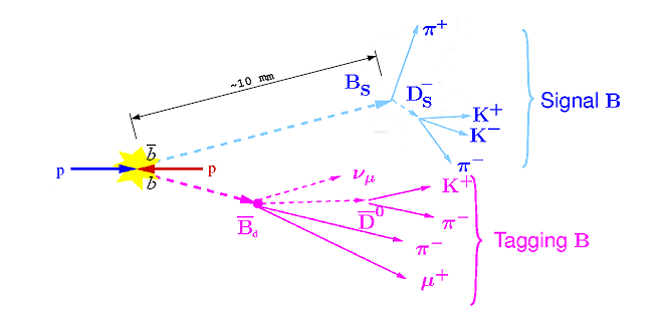
\includegraphics[width=0.6\textwidth]{rysunki/collision.png}
 \caption{Przykład produkcji i rozpadu mezonów pięknych. W produkcji $b\bar{b}$ w eksperymencie LHCb jeden z mezonów \textit{B} traktowany jest jako sygnał, natomiast drugi służy do tzw. znakowania (\textit{tagging B}).}
\end{figure}
\\
\noindent
Śladowy detektor wierzchołka VELO w obrębie którego zachodzi zarówno zderzenie proton-proton jak i rozpad mezonów \textit{B} umożliwia precyzyjny pomiar parametrów pierwotnego wierzchołka oddziaływania jak i wierzchołków wtórnych. Precyzja pomiaru parametru zderzenia z użyciem detektora VELO sięga 20 $\mu m$ dla śladów o wysokim pędzie poprzecznym, zaś precyzja pomiaru położenia w obrębie tego detektora wynosi 42 $\mu m$ na osi $\hat{z}$ i 10 $\mu m$ dla położenia poprzecznego w płaszczyźnie $\hat{x}\hat{y}$.
\\\\
\noindent
Rekonstrukcja nawet częściowa śladów dla przypadku nie jest dostępna na poziomie L0, jednakże dla wysokiego stopnia systemu wyzwalania istnieje możliwość korzystania z częściowej rekonstrukcji śladów. Ze względu na czas wymagany do zrekonstruowania śladów na poziomie HLT analiza i odrzucanie przypadków jest wykonywana sekwencyjnie najpierw w oparciu o ślady dwuwymiarowe w płaszczyźnie $\hat{r}\hat{z}$, następnie w oparciu o ślady trójwymiarowe (sekwencja ta jest opisana w schemacie alei HLT, obrazuje ją rysunek 2.4). Po wykonaniu cięć na parametry zderzenia dla śladów dwu i trójwymiarowych (celem obniżenia częstotliwości przypadków przychodzących do dalszej analizy) możliwa jest rekonstrukcja wybranych śladów, które przechodzą przez pole magnetyczne i dają sygnał w stacjach detektorowych T1-T3. Rekonstrukcja tzw. długich śladów z użyciem stacji T umożliwia pomiar pędu cząstki zostawiającej ślad (po przejściu przez pole magnetyczne) z dokładnością 1\%, przy czym charakterystyczny dla cząstek z rozpadów \textit{B} duży pęd poprzeczny umożliwia wykonanie cięcia dla alei HLT.
\\\\
\noindent
Dla alei fotonowej oba brane pod uwagę kanały rozpadu ($B^{0}_{s}\rightarrow \phi(K^{+}K^{-})\gamma$ oraz $B^{0}_{d}\rightarrow K^{*0}(K^{+}\pi^{-})\gamma$) zawierają dwa mezony o przeciwnych znakach dla których ślady o znaczącym parametrze zderzenia jak i dużym pędzie poprzecznym powinniśmy obserwować w detektorze. Neutralne mezony $\phi$ i $K^{*0}$, oba o masie około 1 GeV, charakteryzują się bardzo krótkim czasem życia, a przebyta przez nie droga nie jest zauważalna w detektorze, dlatego też dla radiacyjnych rozpadów \textit{B} widzimy tylko dwa mezony jako produkty ich rozpadu. Mezony te są produkowane w punkcie rozpadu mezonów $B$ i $B_s$. W wybranych do analizy przypadkach sygnałowych w pełnej rekonstrukcji  zastosowano jedynie cięcie na parametr zderzenia ($IP/\sigma(IP) > 5$), bez cięcia na pęd poprzeczny śladów. W HLT istnieje możliwość obliczenia parametrów zderzenia dwu i trójwymiarowych śladów, jednakże bez znajomości ich błędu co oznacza, iż nie można na poziomie alei wykonać analogicznego cięcia. Przykładową rekonstrukcję śladów 2D w detektorze VELO przedstawia rysunek 3.9
\begin{figure}[!h]
 \centering
 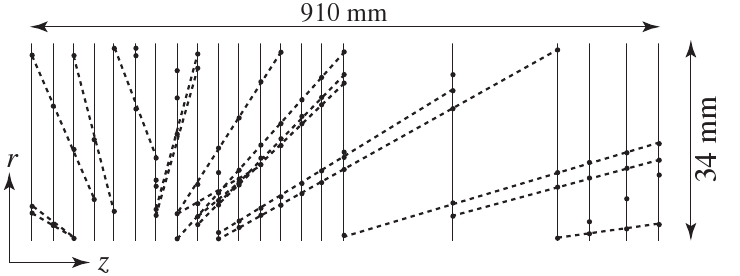
\includegraphics[width=0.8\textwidth]{rysunki/2d.png}
 \caption{Rekonstrukcja dwuwymiarowych śladów w rzucie r-z detektora VELO.}
\end{figure}
\\
\noindent
Ogólna koncepcja alei wysokiego poziomu trygera zakłada cięcie na parametrze zderzenia dwuwymiarowych śladów w granicach 0.1 - 3 mm. Tylko tak wyselekcjonowane ślady mogą być rekonstruowane w trzech wymiarach z powodu ograniczenia czasu wykonania na tym etapie. Rysunek 3.10 przedstawia dwuwymiarowe i trójwymiarowe parametry zderzenia obliczone na podstawie trafień w detektor VELO, dla sygnałowych kaonów z rozpadu $B_s\rightarrow \phi\gamma$.
\begin{figure}[!h]
 \centering
 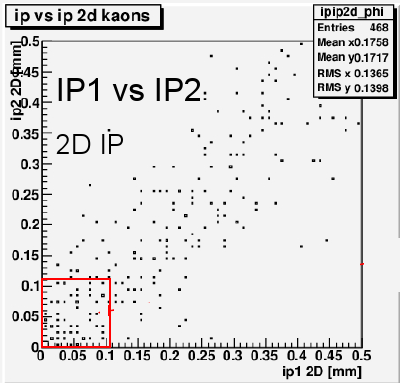
\includegraphics[width=0.42\textwidth]{rysunki/ip2d.png}
 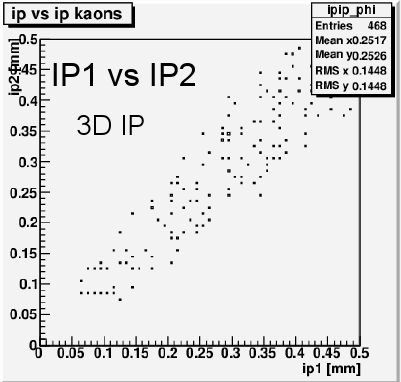
\includegraphics[width=0.42\textwidth]{rysunki/ip3d.png}
 \caption{Obrazek po lewej stronie przedstawia parametry zderzenia sygnałowych mezonów $K^+K^-$ liczone w dwóch wymiarach. Prawy obrazek ilustruje parametry zderzenia liczone dla tych samych śladów w trzech wymiarach.}
\end{figure}
\\
\noindent
Obszar zaznaczony kwadratem dla dwuwymiarowych śladów pokazuje region, dla którego przypadki sygnałowe zostaną odrzucone na tym etapie selekcji. W rzeczywistości oznacza to, że samo cięcie na dwuwymiarowy parametr zderzenia przechodzi 93\% przypadków sygnału i 60\% przypadków tła wpadających do alei (wystarczy znaleźć jeden ślad o parametrze zderzenia w wybranym przedziale). Ponieważ dla przypadków sygnałowych zawsze powinniśmy rekonstruować dwa ślady o podobnych parametrach, cięcie na przynajmniej dwa ślady w zadanym przedziale daje wydajność 92,2\% dla sygnału i 56\% dla tła. Należy pamiętać, że ślady dwuwymiarowe dla HLT są rekonstruowane w oparciu o połowę trafień w płytki detektora VELO (wynika to z konstrukcji detektora VELO, gdzie co druga płytka mierzy odległość $\hat{r}$ od osi detektora), w dodatku informacja o położeniu trafienia jest uzyskiwana jako średnia współrzędnych trafionych pasków detektora Velo, a nie jak w przypadku dokładniejszej rekonstrukcji w oparciu o średnią ważoną. Ma to wpływ na obniżenie jakości wyniku parametru zderzenia co przekłada się na obniżenie efektywności rekonstrukcji. Najważniejszym elementem jest fakt, że na tym etapie zarówno pierwotny wierzchołek oddziaływania jak i parametry zderzenia są rekonstruowane w dwóch wymiarach. Efekt obniżonej efektywności cięcia na parametrze zderzenia śladów dwuwymiarowych jest znanym efektem widocznym także dla innych alei HLT.
\\\\
\noindent
W następnej kolejności wykonuje się cięcie na trójwymiarowy parametr zderzenia w granicach 0.15 - 3 mm, a także wymagane jest aby wybrane na podstawie parametru zderzenia (2D i 3D) ślady były rekonstruowane w stacjach T umieszczonych za magnesem (pole magnetyczne powoduje, że cząstki o niskim pędzie poniżej 2 GeV są wyrzucane poza obręb detektora i nie zostawiają śladów w stacjach T). Powyższe cięcie na parametr zderzenia w trzech wymiarach jak też wymaganie rekonstrukcji śladu w stacjach T nie zmienia znacząco efektywności dla sygnału i tła. Po takiej sekwencji cięć, dla dwóch śladów spełniających powyższe kryteria, efektywność dla sygnału wynosi 91\% przy dwukrotnym obniżeniu poziomu tła (50\%). Dotychczasowe cięcia na parametry śladów w przypadku są standardowymi cięciami dla alei HLT. Uwarunkowane są one ogólnymi cechami rozpadów mezonów \textit{B} oraz ograniczeniami czasowymi wykonania dla wysokiego stopnia trygera, dlatego też w pracy tej nie będą rozważane zmiany sekwencji cięć na parametr zderzenia. 
\\\\
\noindent
W pierwszej realizacji alei fotonowej HLT zastosowano cięcie na jeden ślad z odpowiednim parametrem zderzenia i o pędzie poprzecznym powyżej 1,3 GeV. Cięcie to, choć obniża tło do poziomu 8\% początkowej ilości przypadków, daje niską efektywność dla sygnału - jedynie 66\%. Dane sygnałowe zostały wyselekcjonowane bez cięcia na pęd lub energię poprzeczną hadronów, dlatego też tak wysokie cięcie odrzuca znaczną część sygnału. Rysunek 3.11 przedstawia pęd poprzeczny sygnałowych kaonów z rozpadu $B_s\rightarrow \phi\gamma$. \\
\begin{figure}[!h]
 \centering
 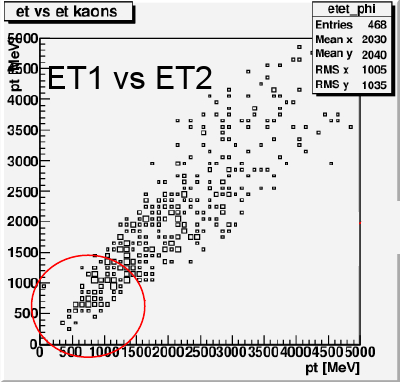
\includegraphics[width=0.5\textwidth]{rysunki/etet.png}
 \caption{Pęd poprzeczny sygnałowych mezonów $K^{+}$ i $K^{-}$.}
\end{figure}
\\
\noindent
Obszar zaznaczony na rysunku 3.11 pokazuje znaczną część przypadków sygnałowych gdzie oba kaony mają energię poprzeczną poniżej 1,2 GeV. Jest to wskazówka, że większą efektywność można uzyskać stosując łagodniejsze cięcie na pęd poprzeczny, ale za to wymagając dwóch takich śladów w każdym przypadku. Tabela 3.3 pokazuje jak zmieniają się efektywności przepuszczania sygnału i tła dla cięcia na pęd poprzeczny jednego lub dwóch śladów jednocześnie wyselekcjonowanych uprzednio parametrem zderzenia.
\begin{table}[!h]
 \centering
 \begin{tabular}{|c|c|c|}
  \hline
  Pęd poprzeczny [MeV] & 1 ślad ef. sygnał/tło [\%] & 2 ślady ef. sygnał/tło [\%] \\
  \hline
   500 &  87,3/30,7 & 80,0/14,0 \\
  \hline
   600 & 85,5/24,4 & 77,0/9,5 \\
  \hline
   700 & 83,3/19,7 & 72,5/6,5 \\
  \hline
   800 & 81,1/16,4 & 67,7/4,7\\
  \hline
   900 & 78,7/13,8 & 64,3/3,7\\
  \hline
  1000 & 75,1/11,9 & 60,9/2,9 \\
  \hline 
  1100 & 71,8/10,7 & 56,4/2,3 \\
  \hline 
  1200 & 68,4/9,3 & 52,4/1,9 \\
  \hline
 \end{tabular}
 \caption{Efektywności cięcia w zależności od pędu poprzecznego śladów.}
\end{table}
\\\\
\noindent
Wyniki umieszczone w tabeli 3.3 pokazują, że przy efektywności dla sygnału ponad 50\% jesteśmy w stanie zredukować poziom tła aż 50-krotnie (2\% efektywności dla przypadków tła), jednocześnie otrzymujemy wtedy bardzo niską efektywność dla przypadków z niskimi pędami poprzecznymi hadronów. Jeśli interesuje nas obniżenie tła ponad 10-krotnie, to większą efektywność dla sygnału uzyskujemy stosując cięcie na dwa ślady (może zaistnieć taka konieczność w celu osiągnięcia sumarycznego 40-krotnego obniżenia poziomu tła). Dla 10-krotnej redukcji tła wydajność dla sygnału jest blisko 10\% wyższa jeśli zastosujemy cięcia na dwa ślady. 
\\\\
\noindent
Powyższa analiza wskazuje na duże możliwości obniżania poziomu tła stosując analizę śladów w oparciu o parametr zderzenia i wysoki pęd poprzeczny charakterstyczne dla produktów rozpadu mezonów \textit{B}. Stosując jedynie warunek na parametr zderzenia tracimy blisko 10\% przypadków sygnałowych co spowodowane jest niewydajnościami szybkiej rekonstrukcji śladów dla HLT. Wnioskiem z obserwacji jest fakt, iż cięcie dla dwóch śladów jednocześnie przy obniżonym progu na pęd poprzeczny daje lepsze rezultaty (blisko 10\% większa wydajność) w porównaniu do analizy tylko jednego śladu (podejście zastosowane w pierwszej implementacji trygera alei fotonowej). Stosunkowo niska wydajność sygnału po zastosowaniu cięć, pomimo iż cięcia nie wykraczają poza rozkłady zmiennych, które sprawdzamy dla cząstek sygnałowych korzystając z informacji MC oraz pełnej rekonstrukcji, spowodowana jest obniżoną jakością wyznaczania parametrów zderzenia śladów dwuwymiarowych na wstępie selekcji. Po niespełnieniu przez sygnałowy ślad warunków dwuwymiarowego parametru zderzenia kolejne cięcia stosowane są do śladów nie pochodzących z sygnału, co przekłada się na niską efektywność całej sekwencji cięć.

\section{Opracowanie sekwencji cięć dla alei fotonowej}

W poprzednich rozdziałach została opisana optymalizacja algorytmów trygera dla poszczególnych charakterystyk sygnałowych rozpadów na poziomie wysokiego stopnia trygera: klastra elektromagnetycznego pochodzącego od sygnałowego fotonu oraz śladów dwóch naładowanych hadronów będących produktami rozpadu mezonów \textit{B}. Podane zostały zoptymalizowane wydajności dla przypadków sygnałowych przy możliwie jak największej redukcji tła analizując oddzielnie klastry w kalorymetrze i ślady. W analizie nie zostały rozpatrzone klastry hadronowe sygnałowych cząstek z powodu ogromnego poziomu tła w kalorymetrze hadronowym dla klastrów o $E_T<1500$ \textit{MeV}. Analiza klastrów hadronowych na poziomie HLT wymagałaby cięcia na $E_T$, którego wykonanie oznaczałoby odrzucenie znaczącej części przypadków sygnałowych. W procesie tworzenia sekwencji cięć należy zwrócić szczególną uwagę, aby nie ustawiać progów dla zmiennych, które w sposób ewidentny odrzucają dane wyselekcjonowane przez pełną rekonstrukcję. Dane sygnałowe zostały wygenerowane w procesie pełnej rekonstrukcji możliwej dla detektora LHCb i nie należy na poziomie trygera ustawiać cięć, które będą wyższe lub nie będą zgodne z cięciami stosowanymi dla pełnej analizy przypadków. Przy konstruowanych w ten sposób cięciach odrzucanie przypadków sygnałowych będzie spowodowane w głównej mierze niewydajnościami w rekonstrukcji dostępnej dla HLT.
\\\\
\noindent
Zadaniem alei fotonowej wysokiego stopnia systemu wyzwalania jest redukcja tła do poziomu 3 kHz, co jest równoznaczne z 40-krotną redukcją w porównaniu z poziomem na wejściu alei, przy możliwie jak największej wydajności dla sygnału. Pierwsza wersja algorytmu alei, będąca pozostałością algorytmu dawnej trzystopniowej wersji trygera, przy efektywności 56\% dla sygnału przepuszczała blisko 8 kHz przypadków tła. Miarą działania wykonywanej optymalizacji jest ulepszenie rezultatów w porównaniu z poprzednią wersją algorytmu. Do dyspozycji mamy separację $merged-\pi^0$/foton, a także ulepszony algorytm cięć dla śladów w przypadku. Zarówno w przypadku klastrów elektromagnetycznych jak i śladów wyniki otrzymane po optymalizacji były lepsze niż dla odpowiadających cięć w pierwszej implementacji alei, dlatego też należy spodziewać się polepszenia działania całego algorytmu alei w oparciu o zoptymalizowane rezultaty.
\\\\
\noindent
Ponieważ z analizy zarówno klastrów elektromagnetycznych jak i śladów wynika, że dla oczekiwanego poziomu tła wydajność alei dla sygnału będzie znacząco odbiegać od 100\%, należy w pierwszej kolejności zastosować cięcia, które w jak najmniejszym stopniu obniżają efektywność sygnału. Dlatego też projekt sekwencji trygera opracowany dla alei fotonowej wygląda następująco (efektywności będą podawane w oparciu o wszystkie poprzednie cięcia łącznie):
\begin{itemize}
 \item podwyższenie progu na energię poprzeczną fotonowego klastra elektromagnetycznego z L0 do poziomu 2,7 GeV. Cięcie to jest analogiczne do zastosowanego w pierwszym stopniu trygera, jednakże dla L0 wynosi ono 2,3 GeV; efektywność dla sygnału wynosi 96,4\%, dla tła 63\%. Cięcie to jest efektywne i w dodatku bardzo proste, ponieważ nie wymaga dodatkowej rekonstrukcji dla HLT,
 \item zastosowanie cięć dla klasyfikatorów otrzymanych z separacji $merged-\pi^0$/foton dla wyselekcjonowanych uprzednio klastrów elektromagnetycznych. Klasyfikatory są różne w zależności od granulacji cel ECal, jednakże średnio otrzymujemy 88,7\% efektywności dla sygnału i 32\% dla tła. Na poziomie klastrów elektromagnetycznych obniżamy trzykrotnie poziom tła (częstotliwość przychodzenia przypadków po analizie w ECal wynosi 40 kHz), 
 \item sekwencja cięć na parametr zderzenia i pęd poprzeczny śladów, wymagane jest zrekonstruowanie dwóch śladów o znaczącym parametrze zderzenia i pędzie poprzecznym powyżej 700 MeV, w rezultacie otrzymujemy żądany poziom tła - 2,97 kHz (2,48\%), oznaczający sumarycznie 40-krotne obniżenie poziomu tła przy 64\% efektywności dla przypadków sygnałowych.
\end{itemize}
\noindent
Tak skonstruowana sekwencja cięć trygera pozwala na implementację wersji algorytmu spełniającej kryterium obniżenia tła do poziomu poniżej 3 kHz. W porównaniu do poprzedniej wersji otrzymujemy ponad dwukrotnie mniejszy poziom tła jednocześnie zwiększając efektywność dla sygnału o 8\%. Sekwencja cięć oraz algorytmy wykorzystywane do analizy przypadków odpowiadają wymaganiom czasowym HLT. Konstrukcja cięcia dla śladów odpowiada standardowemu podejściu dla każdej alei wysokiego stopnia trygera, a jedynym odstępstwem mogącym nie spełniać wymagania czasowego jest szybka rekonstrukcja klastrów elektromagnetycznych w ECal wymagana do separacji $merged-\pi^0$/foton. Jednakże rekonstrukcja taka dla jednego lub dwóch klastrów w przypadku jest możliwa dla alei HLT i nie wykracza poza dostępne ramy czasowe wykonania. Wydajność sygnału na poziomie 64\% jest spowodowana następującymi przyczynami:
\begin{itemize}
 \item dla klastrów elektromagnetycznych z powodu dużego tła od klastrów $\pi^0$ maksymalne obniżenie poziomu przypadków \textit{minimum bias} wynosi 32\%. Efekt ten wymaga skuteczniejszego obniżenia poziomu tła dla podukładu hadronowego,
 \item żadanie ponad 10-krotnego obniżenia tła przy pomocy sekwencji cięć dla śladów wymaga jednocześnie odrzucenia znaczącej części przypadków sygnałowych.
\end{itemize}
\noindent
Stosowanie ostrzejszego cięcia dla klastrów elektromagnetycznych celem większego obniżenia tła, jednocześnie zmniejszając wymagania dla śladów daje znacząco gorsze rezultaty. Otrzymany punkt pracy sekwencji cięć jest zoptymalizowanym rezultatem pod względem wydajności algorytmu dla sygnałowych rozpadów \textit{B} z fotonem.
\\\\
\noindent
Na ostateczny wynik można popatrzeć także z innej strony. Dostosowując cięcia do początkowego poziomu przepuszczania tła przez aleję fotonową - 8 kHz, stosując analogiczną sekwencję przy obniżonych cięciach możemy uzyskać 75\% efektywności dla sygnału. Oznacza to, że optymalizacja algorytmów dla śladów i klastrów elektromagnetycznych pozawala na zwiększenie wydajności alei o blisko 20\% przy takim samym poziomie akceptacji tła.

\chapter{Podsumowanie}
\addcontentsline{toc}{chapter}{Podsumowanie}
Omawiana w pracy aleja fotonowa wysokiego stopnia systemu wyzwalania eksperymentu LHCb została przedstawiona głównie pod kątem wyników i analizy danych. W pracy nie zostały przedstawione szczegóły techniczne dotyczące korzystania z pakietów DaVinci (analiza danych) oraz HLT (wysoki stopień trygera) z oficjalnego oprogramowania LHCb w celu uzyskania interesujących informacji o przypadkach. Wyniki dotyczące wydajności algorytmów zostały otrzymane dla emulacji rzeczywistego działania HLT. Emulacja działania alei jest odtworzeniem rzeczywistego działania algorytmu (takie same zmienne będą dostępne w HLT), dlatego też otrzymane wyniki są wiarygodnym przewidywaniem działania algorytmu dla eksperymentu LHCb. Dla zmiennych opisujących kształt kaskad elektromagnetycznych oraz dla parametrów zderzenia śladów wartości liczbowe zostały obliczone bezpośrednio z odczytu odpowiednich części detektora. Zmienne te trzeba wyznaczyć w czasie rekonstrukcji w HLT, gdyż nie są one dostępne w momencie przyjścia częściowo zrekonstruowanego przypadku do analizy. Analiza dla klastrów elektromagnetycznych była przeprowadzana oddzielnie od analizy śladów w przypadku ze względu na znikomą korelację obu charakterystyk sygnału. Sumaryczna efektywność alei, gdzie stosujemy zarówno cięcia dla klastrów jak i dla śladów, odpowiada przemnożeniu efektywności otrzymanych w oddzielnych analizach dla takich samych cięć. Potwierdza to niezależność obu podukładów dostępnych w alei: fotonu i dwóch śladów (foton ma bardzo słabą rozdzielczość przy wierzchołku rozpadu mezonu \textit{B}).
\\\\
\noindent
Aleja fotonowa, której celem jest osiągnięcie jak najlepszej wydajności dla przypadków zawierających rozpady $B^{0}_{s}\rightarrow \phi\gamma\rightarrow K^{+}K^{-}\gamma$ oraz $B^{0}_{d}\rightarrow K^{*0}\gamma\rightarrow K^{+}\pi^{-}\gamma$ okazała się być trudnym algorytmem, dla którego selekcja przypadku w oparciu o charakterystyki sygnałowe nie zawsze jest możliwa w 100\% dla HLT ze względu na ograniczony czas wykonania. Analiza klastra fotonowego w kalorymetrze elektromagnetycznym, będącego najbardziej charakterystyczną cechą radiacyjnych rozpadów mezonów \textit{B}, nie pozwala na duża redukcję przypadków \textit{minimum bias} z powodu znaczącego tła, w praktyce nieodróżnialnego od sygnału. Klaster elektromagnetyczny jest jedynym efektem istnienia fotonu w rozpadzie, dlatego też do wykorzystania mamy jedynie analizę w oparciu o dane z kalorymetru elektromagnetycznego, która została wykonana. Niecodziennym podejściem jest stosowanie wielowymiarowej analizy bezpośrednio do trygera, jednakże w przypadku separacji $merged-\pi^0$/foton jest to możliwe. Wykorzystany do algorytmu alei jest jedynie klasyfikator otrzymany z próbek danych dla sygnału i tła. Wykorzystano do tego metodę Fishera, która jest metodą prostą i szybką zawierającą bardzo niewiele paramterów\footnote{Liczba parametrów używana w celu obliczenia klasyfikatora jest równa liczbie zmiennych dla których wykonujemy separację. W przypadku separacji $merged-\pi^0$/foton zmiennych do separacji jest 5. Szczegóły metody Fishera opisane są w dodatku do pracy.}. Podejście takie okazało się optymalne i wykazało możliwość separacji cząstek tylko na podstawie informacji o kształcie ich klastrów. W przypadku śladów analiza danych uwidoczniła niewydajności rekonstrukcyjne na poziomie HLT. Analogicznie konstruowana analiza z wykorzystaniem pełnej rekonstrukcji śladów na poziomie \textit{offline} w przypadku pozwala osiągnąć blisko 84\% efektywności dla sygnału przy żądanym poziomie tła. Efektywność po analizie klastrów wynosi 88,7\%, także strata spowodowana cięciem na ślady jest bardzo niewielka. Wskazuje to na zgubienie części informacji podczas rekonstrukcji śladów dwuwymiarowych dla wysokiego stopnia trygera. Ślady dostępne po pełnej rekonstrukcji przypadków charakteryzują się znacznie wyższą precyzją i jakością niż te dostępne w HLT.
\\\\
\noindent
Pomimo trudności w separacji sygnału (radiacyjnych rozpadów mezonów \textit{B}) od tła, otrzymane algorytmy stanowią znaczną poprawę w stosunku do pierwotnej wersji trygera. Dla docelowej konstrukcji alei przy ponad dwukrotnym obniżeniu poziomu tła z 8 do 3 kHz efektywność sygnału została zwiększona z 56\% do 64\% w stosunku do pierwotnej wersji. Przy utrzymaniu takiego samego poziomu tła ośmiu kiloherców, przy pomocy opracowanych algorytmów możemy uzyskać 75\% efektwyności, co daje wynik o ponad 19\% lepszy od początkowego stanu. Większość algorytmów opisanych w pracy zostanie wprowadzona do oficjalnego oprogramowania eksperymentu LHCb w pakiecie HLT.

\newpage
\addcontentsline{toc}{chapter}{Dodatek A - Metoda Fishera separacji danych}
\noindent
\huge{\textbf{Dodatek A - Metoda Fishera separacji danych}}
\normalsize
\\\\\\
\noindent
W metodzie Fishera selekcja przypadków opiera się na liniowej transformacji zmiennych wejściowych poprzez odpowiednio obliczone współczynniki. Następnie decyzja jest podejmowana na podstawie rozkładów sygnału i tła w nowej przestrzeni zmiennych po transformacji.
\\\\
\noindent
Klasyfikacja przypadków opiera się na następujących charakterystykach: średnie zmiennych dla całej próbki $\bar{x}_k$, gdzie $k=1,...,n_{vars}$, średnie tych samych zmiennych w zależności od klasy próbki (sygnał, tło) $\bar{x}_{S(B),k}$, oraz całkowitą macierz kowariancji próbki. Macierz kowariancji można zapisać jako sumę macierzy kowariancji $W$ wewnątrz klasy (sygnał, tło) i $B$ pomiędzy klasami. Macierze te odpowiadają dyspersji przypadków wokół średniej wewnątrz klasy (W), oraz dyspersji wokół średniej całej próbki (B)\footnote{
\noindent
Macierz pomiędzy klasami otrzymywana jest w poniższy sposób:
\[
 W_{kl}=\sum_{U=S(B)}\langle x_{U,k}-\bar{x}_k\rangle \langle x_{U,l}-\bar{x}_l\rangle = C_{S,kl} + C_{B,kl},
\]
gdzie $C_{S(B)}$ jest macierzą kowariancji próbki z sygnału lub tła. Macierz pomiędzy klasami wyraża się:
\[
 B_{kl}=\frac{1}{2}\sum_{U=S(B)}(\bar{x}_{U,k} - \bar{x}_{k})(\bar{x}_{U,l} - \bar{x}_{l}),
\]
gdzie $\bar{x}_{S(B),k}$ jest średnią zmiennej $k$ dla sygnału lub tła, a $\bar{x}_{k}$ jest średnią zmiennej $k$ dla całej próbki.
}.
\\\\
\noindent
Współczynniki Fishera są otrzymywane ze wzoru:
\[
 F_k=\frac{\sqrt{N_{s}N_{b}}}{N_s+N_b}\sum_{l=1}^{n_{vars}}W_{kl}^{-1}\left(\bar{x}_{S,l}-\bar{x}_{B,l}\right),
\]
\noindent
gdzie $N_{S(B)}$ oznaczają liczbę przypadków sygnału i tła w próbce testowej. Dyskryminanta Fishera dla $i$-tego przypadku jest obliczana według wzoru:
\[
 y_{Fi}(i) = F_0 + \sum_{k=1}^{n_{vars}} F_k x_k(i).
\]
\noindent
Istnieje także odmiana metody gdzie współczynniki Fishera są obliczane w oparciu o macierz C - macierz kowariancji wszystkich przypadków (tzw. metoda Mahalanobisa).
\[
 F_k=\frac{\sqrt{N_{s}N_{b}}}{N_s+N_b}\sum_{l=1}^{n_{vars}}C_{kl}^{-1}\left(\bar{x}_{S,l}-\bar{x}_{B,l}\right),
\]
\noindent
gdzie $C_{kl}=B_{kl} + W_{kl}$.
\\\\
\noindent
Klasyfikator otrzymany dla każdego przypadku jest liniową funkcją wejściowych zmiennych. Ma on za zadanie utworzyć zbiory w nowej przestrzeni $y(i)$ tak, aby przypadki z tej samej klasy (sygnał, tło) znajdowały się blisko siebie, a jednocześnie przypadki z odrębnych klas jak najdalej. Wynika to z zastosowania macierzy kowariancji zmiennych wewnątrz klas do obliczenia współczynników Fishera.
\\\\
\noindent
Metoda Fishera, będąca bardzo prostym do implementacji algorytmem, efektywnością nie ustępuje innym bardziej wymagającym metodom separacji danych typu sygnał-tło. Metoda ta jest optymalna dla gausowskich rozkładów zmiennych z liniową korelacją, zaś zupełnie nie funkcjonuje gdy średnie rozkładów sygnału i tła są takie same, a rozkłady różnią się jedynie kształtem.


\begin{thebibliography}{99}
\addcontentsline{toc}{chapter}{Bibliografia}

\bibitem[1]{Szczekowski} Marek Szczekowski, \textit{LHCb - nowy eksperyment do badania naruszania parzystości CP w rozpadach kwarków pięknych}, Postępy Fizyki, Tom 52 (2001) , zeszyt 6.
\bibitem[2]{Lesya} Lesya Shchutska, Andrey Golutvin, Ivan Belayev, \textit{Study of radiative penguin decays $B^{0}\rightarrow K^{*0}\gamma$ and $B^{0}_{s}\rightarrow \phi\gamma$ at LHCb}, LHCb-PHYS-2007-030.
\bibitem[3]{tritdr} \textit{LHCb Trigger System Technical Design Report}, CERN LHCC 2003-031, LHCb TDR 10.
\bibitem[4]{tdr} \textit{LHCb Reoptimized Detector Design and Performance Technical Design Report}, CERN LHCC 2003-030, LHCb TDR 9.
\bibitem[5]{pi0gamma} Sergey Barsuk, CERN/ITEP Moscow, \textit{$\gamma/\pi^0$ separation at high $E_T$}, LHCb week, Calo Software Meeting 20.05.2003
\bibitem[6]{TMVA} \textit{TMVA - Toolkit for Multivariate Data Analysis with ROOT, Users Guide}, arXiv/physics/0703039, CERN-OPEN-2007-007
\end{thebibliography}

\end{document}

